\PassOptionsToPackage{unicode=true}{hyperref} % options for packages loaded elsewhere
\PassOptionsToPackage{hyphens}{url}
%
\documentclass[12pt,]{article}
\usepackage[]{mathpazo}
\usepackage{setspace}
\setstretch{2}
\usepackage{amssymb,amsmath}
\usepackage{ifxetex,ifluatex}
\usepackage{fixltx2e} % provides \textsubscript
\ifnum 0\ifxetex 1\fi\ifluatex 1\fi=0 % if pdftex
  \usepackage[T1]{fontenc}
  \usepackage[utf8]{inputenc}
  \usepackage{textcomp} % provides euro and other symbols
\else % if luatex or xelatex
  \usepackage{unicode-math}
  \defaultfontfeatures{Ligatures=TeX,Scale=MatchLowercase}
\fi
% use upquote if available, for straight quotes in verbatim environments
\IfFileExists{upquote.sty}{\usepackage{upquote}}{}
% use microtype if available
\IfFileExists{microtype.sty}{%
\usepackage[]{microtype}
\UseMicrotypeSet[protrusion]{basicmath} % disable protrusion for tt fonts
}{}
\IfFileExists{parskip.sty}{%
\usepackage{parskip}
}{% else
\setlength{\parindent}{0pt}
\setlength{\parskip}{6pt plus 2pt minus 1pt}
}
\usepackage{hyperref}
\hypersetup{
            pdftitle={Results: Candidate Choice Conjoint},
            pdfauthor={Tiago Ventura},
            pdfborder={0 0 0},
            breaklinks=true}
\urlstyle{same}  % don't use monospace font for urls
\usepackage[margin=1in]{geometry}
\usepackage{color}
\usepackage{fancyvrb}
\newcommand{\VerbBar}{|}
\newcommand{\VERB}{\Verb[commandchars=\\\{\}]}
\DefineVerbatimEnvironment{Highlighting}{Verbatim}{commandchars=\\\{\}}
% Add ',fontsize=\small' for more characters per line
\usepackage{framed}
\definecolor{shadecolor}{RGB}{248,248,248}
\newenvironment{Shaded}{\begin{snugshade}}{\end{snugshade}}
\newcommand{\AlertTok}[1]{\textcolor[rgb]{0.94,0.16,0.16}{#1}}
\newcommand{\AnnotationTok}[1]{\textcolor[rgb]{0.56,0.35,0.01}{\textbf{\textit{#1}}}}
\newcommand{\AttributeTok}[1]{\textcolor[rgb]{0.77,0.63,0.00}{#1}}
\newcommand{\BaseNTok}[1]{\textcolor[rgb]{0.00,0.00,0.81}{#1}}
\newcommand{\BuiltInTok}[1]{#1}
\newcommand{\CharTok}[1]{\textcolor[rgb]{0.31,0.60,0.02}{#1}}
\newcommand{\CommentTok}[1]{\textcolor[rgb]{0.56,0.35,0.01}{\textit{#1}}}
\newcommand{\CommentVarTok}[1]{\textcolor[rgb]{0.56,0.35,0.01}{\textbf{\textit{#1}}}}
\newcommand{\ConstantTok}[1]{\textcolor[rgb]{0.00,0.00,0.00}{#1}}
\newcommand{\ControlFlowTok}[1]{\textcolor[rgb]{0.13,0.29,0.53}{\textbf{#1}}}
\newcommand{\DataTypeTok}[1]{\textcolor[rgb]{0.13,0.29,0.53}{#1}}
\newcommand{\DecValTok}[1]{\textcolor[rgb]{0.00,0.00,0.81}{#1}}
\newcommand{\DocumentationTok}[1]{\textcolor[rgb]{0.56,0.35,0.01}{\textbf{\textit{#1}}}}
\newcommand{\ErrorTok}[1]{\textcolor[rgb]{0.64,0.00,0.00}{\textbf{#1}}}
\newcommand{\ExtensionTok}[1]{#1}
\newcommand{\FloatTok}[1]{\textcolor[rgb]{0.00,0.00,0.81}{#1}}
\newcommand{\FunctionTok}[1]{\textcolor[rgb]{0.00,0.00,0.00}{#1}}
\newcommand{\ImportTok}[1]{#1}
\newcommand{\InformationTok}[1]{\textcolor[rgb]{0.56,0.35,0.01}{\textbf{\textit{#1}}}}
\newcommand{\KeywordTok}[1]{\textcolor[rgb]{0.13,0.29,0.53}{\textbf{#1}}}
\newcommand{\NormalTok}[1]{#1}
\newcommand{\OperatorTok}[1]{\textcolor[rgb]{0.81,0.36,0.00}{\textbf{#1}}}
\newcommand{\OtherTok}[1]{\textcolor[rgb]{0.56,0.35,0.01}{#1}}
\newcommand{\PreprocessorTok}[1]{\textcolor[rgb]{0.56,0.35,0.01}{\textit{#1}}}
\newcommand{\RegionMarkerTok}[1]{#1}
\newcommand{\SpecialCharTok}[1]{\textcolor[rgb]{0.00,0.00,0.00}{#1}}
\newcommand{\SpecialStringTok}[1]{\textcolor[rgb]{0.31,0.60,0.02}{#1}}
\newcommand{\StringTok}[1]{\textcolor[rgb]{0.31,0.60,0.02}{#1}}
\newcommand{\VariableTok}[1]{\textcolor[rgb]{0.00,0.00,0.00}{#1}}
\newcommand{\VerbatimStringTok}[1]{\textcolor[rgb]{0.31,0.60,0.02}{#1}}
\newcommand{\WarningTok}[1]{\textcolor[rgb]{0.56,0.35,0.01}{\textbf{\textit{#1}}}}
\usepackage{graphicx,grffile}
\makeatletter
\def\maxwidth{\ifdim\Gin@nat@width>\linewidth\linewidth\else\Gin@nat@width\fi}
\def\maxheight{\ifdim\Gin@nat@height>\textheight\textheight\else\Gin@nat@height\fi}
\makeatother
% Scale images if necessary, so that they will not overflow the page
% margins by default, and it is still possible to overwrite the defaults
% using explicit options in \includegraphics[width, height, ...]{}
\setkeys{Gin}{width=\maxwidth,height=\maxheight,keepaspectratio}
\setlength{\emergencystretch}{3em}  % prevent overfull lines
\providecommand{\tightlist}{%
  \setlength{\itemsep}{0pt}\setlength{\parskip}{0pt}}
\setcounter{secnumdepth}{0}
% Redefines (sub)paragraphs to behave more like sections
\ifx\paragraph\undefined\else
\let\oldparagraph\paragraph
\renewcommand{\paragraph}[1]{\oldparagraph{#1}\mbox{}}
\fi
\ifx\subparagraph\undefined\else
\let\oldsubparagraph\subparagraph
\renewcommand{\subparagraph}[1]{\oldsubparagraph{#1}\mbox{}}
\fi

% set default figure placement to htbp
\makeatletter
\def\fps@figure{htbp}
\makeatother

\usepackage{booktabs}
\usepackage{amsmath}
\hypersetup{colorlinks,citecolor=blue,filecolor=red,linkcolor=brown,urlcolor=blue}
\usepackage{lmodern}
\usepackage[shadow,roundedcorners,customcolors]{dynblocks}
\usepackage{natbib}
\usepackage[utf8]{inputenc}

\title{Results: Candidate Choice Conjoint}
\author{Tiago Ventura}
\date{}

\begin{document}
\maketitle

\hypertarget{introduction}{%
\section{Introduction}\label{introduction}}

In this short report, I present the main results for the Conjoint
Experiment on Candidate Choice and Security Policies in Mexico.

\hypertarget{cleaning-and-preparing-the-data}{%
\subsection{Cleaning and Preparing the
data}\label{cleaning-and-preparing-the-data}}

\begin{Shaded}
\begin{Highlighting}[]
\CommentTok{# Functions ---------------------------------------------------------------}


\CommentTok{# short view}
\NormalTok{short_view <-}\StringTok{ }\ControlFlowTok{function}\NormalTok{(data)\{}
\NormalTok{  data }\OperatorTok\StringTok{ }\KeywordTok{slice}\NormalTok{(}\DecValTok{1}\OperatorTok{:}\DecValTok{50}\NormalTok{) }\OperatorTok\StringTok{ }\KeywordTok{View}\NormalTok{()}
\NormalTok{\}}

\CommentTok{# ggplot theme ------------------------------------------------------------}
\CommentTok{#my_font <- "Palatino Linotype"}
\NormalTok{my_bkgd <-}\StringTok{ "white"}
\CommentTok{#my_bkgd <- "#f5f5f2"}
\NormalTok{pal <-}\StringTok{ }\NormalTok{RColorBrewer}\OperatorTok{::}\KeywordTok{brewer.pal}\NormalTok{(}\DecValTok{9}\NormalTok{, }\StringTok{"Spectral"}\NormalTok{)}


\NormalTok{my_theme <-}\StringTok{ }\KeywordTok{theme}\NormalTok{(}\DataTypeTok{text =} \KeywordTok{element_text}\NormalTok{(}\DataTypeTok{color =} \StringTok{"#22211d"}\NormalTok{),}
                  \DataTypeTok{rect =} \KeywordTok{element_rect}\NormalTok{(}\DataTypeTok{fill =}\NormalTok{ my_bkgd),}
                  \DataTypeTok{plot.background =} \KeywordTok{element_rect}\NormalTok{(}\DataTypeTok{fill =}\NormalTok{ my_bkgd, }\DataTypeTok{color =} \OtherTok{NA}\NormalTok{),}
                  \DataTypeTok{panel.background =} \KeywordTok{element_rect}\NormalTok{(}\DataTypeTok{fill =}\NormalTok{ my_bkgd, }\DataTypeTok{color =} \OtherTok{NA}\NormalTok{),}
                  \DataTypeTok{panel.border =} \KeywordTok{element_rect}\NormalTok{(}\DataTypeTok{color=}\StringTok{"black"}\NormalTok{), }
                  \DataTypeTok{strip.background =} \KeywordTok{element_rect}\NormalTok{(}\DataTypeTok{color=}\StringTok{"black"}\NormalTok{, }\DataTypeTok{fill=}\StringTok{"gray85"}\NormalTok{), }
                  \DataTypeTok{legend.background =} \KeywordTok{element_rect}\NormalTok{(}\DataTypeTok{fill =}\NormalTok{ my_bkgd, }\DataTypeTok{color =} \OtherTok{NA}\NormalTok{),}
                  \DataTypeTok{legend.key.size =} \KeywordTok{unit}\NormalTok{(}\DecValTok{1}\NormalTok{, }\StringTok{"cm"}\NormalTok{),}
                  \DataTypeTok{legend.text =} \KeywordTok{element_text}\NormalTok{(}\DataTypeTok{size =} \DecValTok{10}\NormalTok{),}
                  \DataTypeTok{legend.title =} \KeywordTok{element_text}\NormalTok{(}\DataTypeTok{size=}\DecValTok{10}\NormalTok{),}
                  \DataTypeTok{plot.title =} \KeywordTok{element_text}\NormalTok{(}\DataTypeTok{size =} \DecValTok{14}\NormalTok{, }\DataTypeTok{face =} \StringTok{"bold"}\NormalTok{),}
                  \DataTypeTok{plot.subtitle =} \KeywordTok{element_text}\NormalTok{(}\DataTypeTok{size=}\DecValTok{12}\NormalTok{),}
                  \DataTypeTok{axis.title.x =} \KeywordTok{element_text}\NormalTok{(}\DataTypeTok{hjust=}\DecValTok{1}\NormalTok{,  }\DataTypeTok{size=}\DecValTok{7}\NormalTok{),}
                  \DataTypeTok{axis.text.y=}\KeywordTok{element_text}\NormalTok{(}\DataTypeTok{size=}\DecValTok{10}\NormalTok{,}\DataTypeTok{hjust=}\DecValTok{0}\NormalTok{),}
                  \DataTypeTok{plot.margin =} \KeywordTok{margin}\NormalTok{(}\DecValTok{1}\NormalTok{, }\DecValTok{1}\NormalTok{, }\DecValTok{1}\NormalTok{, }\DecValTok{1}\NormalTok{, }\StringTok{"cm"}\NormalTok{))}





\CommentTok{# Download the data -------------------------------------------------------}

\KeywordTok{load}\NormalTok{(}\StringTok{"./data/mexico_cleaned2_data.Rdata"}\NormalTok{)}

\KeywordTok{dim}\NormalTok{(d)}
\end{Highlighting}
\end{Shaded}

\begin{verbatim}
[1] 2346  331
\end{verbatim}

\begin{Shaded}
\begin{Highlighting}[]
\CommentTok{# Check Covariates --------------------------------------------------------}

\CommentTok{#levels(d$education)}
\CommentTok{#class(d$income)}
\CommentTok{#levels(d$work)}
\CommentTok{#levels(d$age)}

\CommentTok{# Cleaning the Conjoints --------------------------------------------------}

\CommentTok{## Putting together the two taks. }

\NormalTok{outcomes <-}\StringTok{ }\NormalTok{d }\OperatorTok\StringTok{ }
\StringTok{          }\KeywordTok{select}\NormalTok{(responseid,conjoint1_outcome, conjoint2_outcome)}

\NormalTok{outcomes <-}\StringTok{ }\NormalTok{outcomes  }\OperatorTok\StringTok{ }
\StringTok{  }\KeywordTok{pivot_longer}\NormalTok{(}\DataTypeTok{cols =} \OperatorTok{-}\NormalTok{responseid, }
               \DataTypeTok{names_to =} \StringTok{"var"}\NormalTok{, }
               \DataTypeTok{values_to =} \StringTok{"outcome"}\NormalTok{) }\OperatorTok\StringTok{ }
\StringTok{  }\KeywordTok{mutate}\NormalTok{(}\DataTypeTok{task=} \KeywordTok{ifelse}\NormalTok{(var}\OperatorTok{==}\StringTok{"conjoint1_outcome"}\NormalTok{, }\StringTok{"choice_1"}\NormalTok{, }\StringTok{"choice_2"}\NormalTok{), }
         \DataTypeTok{candidate=} \KeywordTok{ifelse}\NormalTok{(outcome}\OperatorTok{==}\StringTok{"Candidato A"}\NormalTok{, }\StringTok{"cd_1"}\NormalTok{, }\StringTok{"cd_2"}\NormalTok{), }
         \DataTypeTok{missing_id=} \KeywordTok{ifelse}\NormalTok{(}\KeywordTok{is.na}\NormalTok{(outcome)}\OperatorTok{|}\NormalTok{outcome}\OperatorTok{==}\StringTok{"-999"}\NormalTok{, }\DecValTok{1}\NormalTok{, }\DecValTok{0}\NormalTok{), }
         \DataTypeTok{candidate=}\KeywordTok{ifelse}\NormalTok{(missing_id}\OperatorTok{==}\DecValTok{1}\NormalTok{, }\StringTok{"cd_1"}\NormalTok{, candidate)) }

\CommentTok{# it doesnt matter, I will exclude the missing}

\CommentTok{#short_view(outcomes)}

\CommentTok{# The features ------------------------------------------------------------}

\CommentTok{### Clean the features}


\CommentTok{### Function to extract the features}

\NormalTok{features <-}\StringTok{ }\NormalTok{d }\OperatorTok\StringTok{ }\KeywordTok{select}\NormalTok{(responseid, }\KeywordTok{matches}\NormalTok{(}\StringTok{"^f_"}\NormalTok{))}
\CommentTok{#View(features)}

\NormalTok{var_feature_}\DecValTok{1}\NormalTok{ <-}\StringTok{ }\KeywordTok{c}\NormalTok{(}\StringTok{"f_1_1"}\NormalTok{, }\StringTok{"f_1_1_1"}\NormalTok{, }\StringTok{"f_1_2_1"}\NormalTok{, }\StringTok{"f_2_1_1"}\NormalTok{, }\StringTok{"f_2_2_1"}\NormalTok{)}
\NormalTok{var_feature_}\DecValTok{2}\NormalTok{ <-}\StringTok{ }\KeywordTok{c}\NormalTok{(}\StringTok{"f_1_2"}\NormalTok{, }\StringTok{"f_1_1_2"}\NormalTok{, }\StringTok{"f_1_2_2"}\NormalTok{, }\StringTok{"f_2_1_2"}\NormalTok{, }\StringTok{"f_2_2_2"}\NormalTok{)}
\NormalTok{var_feature_}\DecValTok{3}\NormalTok{ <-}\StringTok{ }\KeywordTok{c}\NormalTok{(}\StringTok{"f_1_3"}\NormalTok{, }\StringTok{"f_1_1_3"}\NormalTok{, }\StringTok{"f_1_2_3"}\NormalTok{, }\StringTok{"f_2_1_3"}\NormalTok{, }\StringTok{"f_2_2_3"}\NormalTok{)}
\NormalTok{var_feature_}\DecValTok{4}\NormalTok{ <-}\StringTok{ }\KeywordTok{c}\NormalTok{(}\StringTok{"f_1_4"}\NormalTok{, }\StringTok{"f_1_1_4"}\NormalTok{, }\StringTok{"f_1_2_4"}\NormalTok{, }\StringTok{"f_2_1_4"}\NormalTok{, }\StringTok{"f_2_2_4"}\NormalTok{)}

\CommentTok{# Function}
\NormalTok{cj_extract_features <-}\StringTok{ }\ControlFlowTok{function}\NormalTok{(data, variables)\{}
\NormalTok{  feature <-}\StringTok{ }\NormalTok{data }\OperatorTok\StringTok{ }\KeywordTok{select}\NormalTok{(responseid,variables)}
\NormalTok{  feature }\OperatorTok\StringTok{ }\KeywordTok{pivot_longer}\NormalTok{(}
    \DataTypeTok{cols =}\NormalTok{ variables[}\OperatorTok{-}\DecValTok{1}\NormalTok{],}
    \DataTypeTok{names_to =} \StringTok{"var"}\NormalTok{,}
    \DataTypeTok{values_to =} \StringTok{"value"}\NormalTok{) }\OperatorTok\StringTok{ }
\StringTok{    }\KeywordTok{mutate}\NormalTok{(}\DataTypeTok{task=}\KeywordTok{ifelse}\NormalTok{(}\KeywordTok{str_detect}\NormalTok{(var, }\StringTok{"f_1"}\NormalTok{),}\StringTok{"choice_1"}\NormalTok{, }\StringTok{"choice_2"}\NormalTok{), }\CommentTok{# extract the task}
           \DataTypeTok{candidate=} \KeywordTok{ifelse}\NormalTok{(}\KeywordTok{str_detect}\NormalTok{(var, DGT }\OperatorTok\StringTok{ "_1_"} \OperatorTok\StringTok{ }\NormalTok{DGT }\OperatorTok\StringTok{ }\NormalTok{END),}\StringTok{"cd_1"}\NormalTok{, }\StringTok{"cd_2"}\NormalTok{))   }\OperatorTok\StringTok{ }
\StringTok{    }\KeywordTok{rename}\NormalTok{(}\StringTok{"features"}\NormalTok{=variables[}\DecValTok{1}\NormalTok{]) }
\NormalTok{\}}


\CommentTok{## Extract}
\NormalTok{list_features <-}\StringTok{ }\KeywordTok{list}\NormalTok{(var_feature_}\DecValTok{1}\NormalTok{, var_feature_}\DecValTok{2}\NormalTok{, var_feature_}\DecValTok{3}\NormalTok{, var_feature_}\DecValTok{4}\NormalTok{)}

\NormalTok{features_long <-}\StringTok{ }\KeywordTok{map_dfr}\NormalTok{(list_features, }\OperatorTok{~}\StringTok{ }\KeywordTok{cj_extract_features}\NormalTok{(d, .x)) }\OperatorTok\StringTok{ }
\StringTok{  }\KeywordTok{drop_na}\NormalTok{(features)}

\NormalTok{features_wider <-}\StringTok{ }\NormalTok{features_long }\OperatorTok\StringTok{ }\KeywordTok{select}\NormalTok{(}\OperatorTok{-}\NormalTok{var) }\OperatorTok
\StringTok{  }\KeywordTok{pivot_wider}\NormalTok{(}
    \DataTypeTok{names_from =}\NormalTok{ features,  }
    \DataTypeTok{values_from=}\NormalTok{ value) }


\CommentTok{### Put together with the outcomes}

\CommentTok{# Invert the merge here. Since I just recorded in the outcome the candidate choosen, }
\CommentTok{# I have to merge by the right, which means preserving the missings from the features data}
\CommentTok{# the missings will be the cases no choosen}

\NormalTok{conjoint_data_to_remove <-}\StringTok{ }\KeywordTok{left_join}\NormalTok{(features_wider,outcomes, }\DataTypeTok{by=}\KeywordTok{c}\NormalTok{(}\StringTok{"responseid"}\NormalTok{, }\StringTok{"task"}\NormalTok{))}
\NormalTok{id_to_remove <-}\StringTok{ }\NormalTok{conjoint_data_to_remove }\OperatorTok\StringTok{ }
\StringTok{  }\KeywordTok{filter}\NormalTok{(missing_id}\OperatorTok{==}\DecValTok{1}\NormalTok{)  }\OperatorTok\StringTok{ }
\StringTok{  }\KeywordTok{select}\NormalTok{(responseid, task, missing_id) }

\CommentTok{# Convert the missings to zero. But first, eliminate the real missings}

\NormalTok{conjoint_data <-}\StringTok{ }\KeywordTok{left_join}\NormalTok{(features_wider,outcomes) }\OperatorTok\StringTok{ }
\StringTok{  }\KeywordTok{anti_join}\NormalTok{(id_to_remove, }\DataTypeTok{by=}\KeywordTok{c}\NormalTok{(}\StringTok{"responseid"}\NormalTok{, }\StringTok{"task"}\NormalTok{)) }\OperatorTok
\StringTok{  }\KeywordTok{mutate}\NormalTok{(}\DataTypeTok{outcome_num=}\KeywordTok{ifelse}\NormalTok{(}\KeywordTok{is.na}\NormalTok{(outcome), }\DecValTok{0}\NormalTok{, }\DecValTok{1}\NormalTok{)) }\OperatorTok
\StringTok{  }\KeywordTok{select}\NormalTok{(}\OperatorTok{-}\NormalTok{var, }\OperatorTok{-}\NormalTok{missing_id)}


\CommentTok{#View(conjoint_data)}

\CommentTok{# Check}
\CommentTok{#table(conjoint_data$outcome_num)}

\CommentTok{# perfect = equal answers}

\KeywordTok{colnames}\NormalTok{(conjoint_data) <-}\StringTok{ }\KeywordTok{c}\NormalTok{(}\StringTok{"responseid"}\NormalTok{, }\StringTok{"task"}\NormalTok{, }\StringTok{"candidate"}\NormalTok{, }
                             \StringTok{"feat_political_party"}\NormalTok{, }
                             \StringTok{"feat_security_proposal"}\NormalTok{, }
                             \StringTok{"feat_occupation"}\NormalTok{, }
                             \StringTok{"feat_gender"}\NormalTok{,}
                             \StringTok{"outcome"}\NormalTok{, }\StringTok{"outcome_num"}\NormalTok{)}


\CommentTok{# Get the baselines}

\CommentTok{# Check Security Policy}

\KeywordTok{library}\NormalTok{(janitor)}
\CommentTok{# conjoint_data %>% tabyl(feat_security_proposal) %>% View()}
\CommentTok{# conjoint_data %>% tabyl(feat_occupation) %>% View()}



\NormalTok{conjoint_data <-}\StringTok{ }\NormalTok{conjoint_data }\OperatorTok\StringTok{ }
\StringTok{  }\KeywordTok{mutate_at}\NormalTok{(}\KeywordTok{vars}\NormalTok{(}\KeywordTok{contains}\NormalTok{(}\StringTok{"feat_"}\NormalTok{)), as_factor) }\OperatorTok
\StringTok{  }\KeywordTok{mutate}\NormalTok{(}\DataTypeTok{feat_political_party=}\KeywordTok{fct_relevel}\NormalTok{(feat_political_party, }\StringTok{"Independiente"}\NormalTok{), }
         \DataTypeTok{feat_gender=}\KeywordTok{fct_relevel}\NormalTok{(feat_gender, }\StringTok{"Mujer"}\NormalTok{), }
         \DataTypeTok{feat_security_proposal=} \KeywordTok{fct_relevel}\NormalTok{(feat_security_proposal, }
                                             \StringTok{"Creaci昼㸳n de un centro de asesor攼㹤a y atenci昼㸳n a v攼㹤ctimas"}\NormalTok{),}
         \DataTypeTok{feat_occupation=} \KeywordTok{fct_relevel}\NormalTok{(feat_occupation, }\StringTok{"Empleado p昼㹡blico"}\NormalTok{))}


\CommentTok{# Combine -----------------------------------------------------------------}

\NormalTok{conjoint_data <-}\StringTok{ }\KeywordTok{left_join}\NormalTok{(d, conjoint_data)}

\CommentTok{#conjoint_data %>% tabyl(feat_occupation, outcome_num)}


\CommentTok{# Rename levels -----------------------------------------------------------}

\CommentTok{# Gender}
\NormalTok{levels_gender <-}\StringTok{ }\KeywordTok{levels}\NormalTok{(conjoint_data}\OperatorTok{$}\NormalTok{feat_gender)}
\NormalTok{levels_gender <-}\StringTok{ }\KeywordTok{list}\NormalTok{(}\StringTok{"Male"}\NormalTok{=}\StringTok{ }\NormalTok{levels_gender[}\DecValTok{2}\NormalTok{], }
                      \StringTok{"Female"}\NormalTok{ =}\StringTok{ }\NormalTok{levels_gender[}\DecValTok{1}\NormalTok{])}

\CommentTok{# Party}

\NormalTok{levels_party <-}\StringTok{ }\KeywordTok{levels}\NormalTok{(conjoint_data}\OperatorTok{$}\NormalTok{feat_political_party)}
\NormalTok{levels_party <-}\StringTok{ }\KeywordTok{list}\NormalTok{(}\StringTok{"PRI"}\NormalTok{=}\StringTok{"PRI"}\NormalTok{, }\StringTok{"MORENA"}\NormalTok{=}\StringTok{"Morena"}\NormalTok{, }\StringTok{"PAN"}\NormalTok{=}\StringTok{"PAN"}\NormalTok{, }
                     \StringTok{"Independents"}\NormalTok{=}\StringTok{"Independiente"}\NormalTok{)}

\CommentTok{# Occupation}
\NormalTok{levels_occup <-}\StringTok{ }\KeywordTok{levels}\NormalTok{(conjoint_data}\OperatorTok{$}\NormalTok{feat_occupation)}
\NormalTok{levels_occup <-}\StringTok{ }\KeywordTok{list}\NormalTok{(}\StringTok{"Leader Autodefensas"}\NormalTok{ =}\StringTok{ }\NormalTok{levels_occup[}\DecValTok{2}\NormalTok{], }
                     \StringTok{"Chief Local Police"}\NormalTok{ =}\StringTok{ }\NormalTok{levels_occup[}\DecValTok{3}\NormalTok{], }
                     \StringTok{"Human-Rights Activist"}\NormalTok{=levels_occup[}\DecValTok{4}\NormalTok{], }
                     \StringTok{"Owner Private  Security Firm"}\NormalTok{=levels_occup[}\DecValTok{5}\NormalTok{], }
                     \StringTok{"Public Employee"}\NormalTok{=levels_occup[}\DecValTok{1}\NormalTok{])}

\CommentTok{# Proposal}
\NormalTok{levels_sec <-}\StringTok{ }\KeywordTok{levels}\NormalTok{(conjoint_data}\OperatorTok{$}\NormalTok{feat_security_proposal)}
\NormalTok{levels_sec <-}\StringTok{ }\KeywordTok{list}\NormalTok{(}\StringTok{"Education to Youth"}\NormalTok{=}\StringTok{ }\NormalTok{levels_sec[}\DecValTok{2}\NormalTok{], }
                  \StringTok{"Better Police/Security Cameras"}\NormalTok{=}\StringTok{ }\NormalTok{levels_sec[}\DecValTok{3}\NormalTok{],}
                  \StringTok{"Death Penalty"}\NormalTok{=}\StringTok{ }\NormalTok{levels_sec[}\DecValTok{4}\NormalTok{],}
                  \StringTok{"Police Militarization"}\NormalTok{=}\StringTok{ }\NormalTok{levels_sec[}\DecValTok{5}\NormalTok{], }
                  \StringTok{"Victims Oriented Policies"}\NormalTok{=}\StringTok{ }\NormalTok{levels_sec[}\DecValTok{1}\NormalTok{])}

\NormalTok{conjoint_data <-}\StringTok{ }\NormalTok{conjoint_data }\OperatorTok\StringTok{ }
\StringTok{                  }\KeywordTok{mutate}\NormalTok{(}\DataTypeTok{feat_gender=}\KeywordTok{fct_recode}\NormalTok{(feat_gender, }\OperatorTok{!!!}\NormalTok{levels_gender), }
                         \DataTypeTok{feat_political_party=}\KeywordTok{fct_recode}\NormalTok{(feat_political_party, }\OperatorTok{!!!}\NormalTok{levels_party), }
                         \DataTypeTok{feat_occupation=}\KeywordTok{fct_recode}\NormalTok{(feat_occupation, }\OperatorTok{!!!}\NormalTok{levels_occup), }
                         \DataTypeTok{feat_security_proposal=}\KeywordTok{fct_recode}\NormalTok{(feat_security_proposal,}
                                                           \OperatorTok{!!!}\NormalTok{levels_sec))}
\end{Highlighting}
\end{Shaded}

\hypertarget{modelling-function}{%
\subsection{Modelling Function}\label{modelling-function}}

\begin{Shaded}
\begin{Highlighting}[]
\CommentTok{# Modeling ----------------------------------------------------------------}
\NormalTok{features =}\StringTok{ }\KeywordTok{c}\NormalTok{(}\StringTok{"political_party"}\NormalTok{, }\StringTok{"gender"}\NormalTok{, }\StringTok{"occupation"}\NormalTok{, }\StringTok{"security_proposal"}\NormalTok{)}
\NormalTok{references <-}\StringTok{ }\KeywordTok{c}\NormalTok{(}\KeywordTok{levels}\NormalTok{(conjoint_data}\OperatorTok{$}\NormalTok{feat_political_party)[}\DecValTok{1}\NormalTok{],}
                \KeywordTok{levels}\NormalTok{(conjoint_data}\OperatorTok{$}\NormalTok{feat_gender)[}\DecValTok{1}\NormalTok{],}
                \KeywordTok{levels}\NormalTok{(conjoint_data}\OperatorTok{$}\NormalTok{feat_occupation)[}\DecValTok{1}\NormalTok{], }
                \KeywordTok{levels}\NormalTok{(conjoint_data}\OperatorTok{$}\NormalTok{feat_security_proposal)[}\DecValTok{1}\NormalTok{])}

\NormalTok{list_terms <-}\StringTok{ }\KeywordTok{c}\NormalTok{(}\StringTok{"Political Party"}\NormalTok{, }\KeywordTok{paste0}\NormalTok{(}\StringTok{"    "}\NormalTok{, }\KeywordTok{names}\NormalTok{(levels_party)), }\StringTok{" "}\NormalTok{,}
                   \StringTok{"Gender"}\NormalTok{, }\KeywordTok{paste0}\NormalTok{(}\StringTok{"    "}\NormalTok{, }\KeywordTok{names}\NormalTok{(levels_gender)),}\StringTok{"  "}\NormalTok{, }
                   \StringTok{"Occupation"}\NormalTok{, }\KeywordTok{paste0}\NormalTok{(}\StringTok{"    "}\NormalTok{, }\KeywordTok{names}\NormalTok{(levels_occup)), }\StringTok{"   "}\NormalTok{,}
                   \StringTok{"Security Proposal"}\NormalTok{, }\KeywordTok{paste0}\NormalTok{(}\StringTok{"    "}\NormalTok{, }\KeywordTok{names}\NormalTok{(levels_sec)), }\StringTok{"    "}\NormalTok{)}

\NormalTok{tidy_conjoint_model <-}\StringTok{ }\ControlFlowTok{function}\NormalTok{(model, subsample, }\DataTypeTok{features=}\NormalTok{features,}
                                \DataTypeTok{references=}\NormalTok{references, list_terms)\{}
  
  \CommentTok{# to make it more general, it is just to change the  4 for the number of features}
\NormalTok{  model }\OperatorTok\StringTok{ }
\StringTok{    }\KeywordTok{tidy}\NormalTok{(.) }\OperatorTok\StringTok{ }
\StringTok{    }\KeywordTok{mutate}\NormalTok{(}\DataTypeTok{lb=}\NormalTok{estimate }\OperatorTok{-}\StringTok{ }\FloatTok{1.96}\OperatorTok{*}\NormalTok{std.error, }
           \DataTypeTok{up=}\NormalTok{ estimate }\OperatorTok{+}\StringTok{ }\FloatTok{1.96}\OperatorTok{*}\NormalTok{std.error, }
           \DataTypeTok{lb90=}\NormalTok{estimate }\OperatorTok{-}\StringTok{ }\FloatTok{1.64}\OperatorTok{*}\NormalTok{std.error, }
           \DataTypeTok{up90=}\NormalTok{ estimate }\OperatorTok{+}\StringTok{ }\FloatTok{1.64}\OperatorTok{*}\NormalTok{std.error) }\OperatorTok\StringTok{ }
\StringTok{    }\KeywordTok{filter}\NormalTok{(}\OperatorTok{!}\NormalTok{(term }\OperatorTok\StringTok{ }\KeywordTok{c}\NormalTok{(}\StringTok{"(Intercept)"}\NormalTok{))) }\OperatorTok\StringTok{ }
\StringTok{    }\KeywordTok{mutate}\NormalTok{(}\DataTypeTok{term=}\KeywordTok{str_remove_all}\NormalTok{(term, }\KeywordTok{paste0}\NormalTok{(}\StringTok{"feat_"}\NormalTok{, features, }\DataTypeTok{collapse =} \StringTok{"|"}\NormalTok{)),}
           \DataTypeTok{term=}\KeywordTok{str_replace_all}\NormalTok{(term, }\StringTok{"_"}\NormalTok{, }\StringTok{" "}\NormalTok{),}
           \DataTypeTok{term=}\KeywordTok{as.factor}\NormalTok{(term), }
           \DataTypeTok{term=}\KeywordTok{str_c}\NormalTok{(}\StringTok{"    "}\NormalTok{, term)) }\OperatorTok
\StringTok{    }\KeywordTok{bind_rows}\NormalTok{(}\KeywordTok{data_frame}\NormalTok{(}\DataTypeTok{term=}\KeywordTok{c}\NormalTok{(}\KeywordTok{str_to_title}\NormalTok{(}\KeywordTok{str_replace_all}\NormalTok{(features, }\StringTok{"_"}\NormalTok{, }\StringTok{" "}\NormalTok{)), }
                                \StringTok{" "}\NormalTok{, }\StringTok{"  "}\NormalTok{, }\StringTok{"   "}\NormalTok{, }\StringTok{"    "}\NormalTok{,}
                                \KeywordTok{paste0}\NormalTok{(}\StringTok{"    "}\NormalTok{, references)), }
                         \DataTypeTok{estimate=}\KeywordTok{c}\NormalTok{(}\KeywordTok{rep}\NormalTok{(}\OtherTok{NA}\NormalTok{, }\DecValTok{4}\NormalTok{), }\KeywordTok{rep}\NormalTok{(}\OtherTok{NA}\NormalTok{, }\DecValTok{4}\NormalTok{), }\KeywordTok{rep}\NormalTok{(}\DecValTok{0}\NormalTok{,}\DecValTok{4}\NormalTok{)),  }
                         \DataTypeTok{std.error=}\KeywordTok{c}\NormalTok{(}\KeywordTok{rep}\NormalTok{(}\OtherTok{NA}\NormalTok{, }\DecValTok{4}\NormalTok{), }\KeywordTok{rep}\NormalTok{(}\OtherTok{NA}\NormalTok{, }\DecValTok{4}\NormalTok{), }\KeywordTok{rep}\NormalTok{(}\DecValTok{0}\NormalTok{,}\DecValTok{4}\NormalTok{)),  }
                         \DataTypeTok{statistic=}\KeywordTok{c}\NormalTok{(}\KeywordTok{rep}\NormalTok{(}\OtherTok{NA}\NormalTok{, }\DecValTok{4}\NormalTok{), }\KeywordTok{rep}\NormalTok{(}\OtherTok{NA}\NormalTok{, }\DecValTok{4}\NormalTok{), }\KeywordTok{rep}\NormalTok{(}\DecValTok{0}\NormalTok{,}\DecValTok{4}\NormalTok{)),  }
                         \DataTypeTok{p.value=}\KeywordTok{c}\NormalTok{(}\KeywordTok{rep}\NormalTok{(}\OtherTok{NA}\NormalTok{, }\DecValTok{4}\NormalTok{), }\KeywordTok{rep}\NormalTok{(}\OtherTok{NA}\NormalTok{, }\DecValTok{4}\NormalTok{), }\KeywordTok{rep}\NormalTok{(}\DecValTok{0}\NormalTok{,}\DecValTok{4}\NormalTok{)), }
                         \DataTypeTok{lb=}\KeywordTok{c}\NormalTok{(}\KeywordTok{rep}\NormalTok{(}\OtherTok{NA}\NormalTok{, }\DecValTok{4}\NormalTok{), }\KeywordTok{rep}\NormalTok{(}\OtherTok{NA}\NormalTok{, }\DecValTok{4}\NormalTok{), }\KeywordTok{rep}\NormalTok{(}\DecValTok{0}\NormalTok{,}\DecValTok{4}\NormalTok{)),  }
                         \DataTypeTok{up=}\KeywordTok{c}\NormalTok{(}\KeywordTok{rep}\NormalTok{(}\OtherTok{NA}\NormalTok{, }\DecValTok{4}\NormalTok{), }\KeywordTok{rep}\NormalTok{(}\OtherTok{NA}\NormalTok{, }\DecValTok{4}\NormalTok{), }\KeywordTok{rep}\NormalTok{(}\DecValTok{0}\NormalTok{,}\DecValTok{4}\NormalTok{)), }
                         \DataTypeTok{lb90=}\KeywordTok{c}\NormalTok{(}\KeywordTok{rep}\NormalTok{(}\OtherTok{NA}\NormalTok{, }\DecValTok{4}\NormalTok{), }\KeywordTok{rep}\NormalTok{(}\OtherTok{NA}\NormalTok{, }\DecValTok{4}\NormalTok{), }\KeywordTok{rep}\NormalTok{(}\DecValTok{0}\NormalTok{,}\DecValTok{4}\NormalTok{)),  }
                         \DataTypeTok{up90=}\KeywordTok{c}\NormalTok{(}\KeywordTok{rep}\NormalTok{(}\OtherTok{NA}\NormalTok{, }\DecValTok{4}\NormalTok{), }\KeywordTok{rep}\NormalTok{(}\OtherTok{NA}\NormalTok{, }\DecValTok{4}\NormalTok{), }\KeywordTok{rep}\NormalTok{(}\DecValTok{0}\NormalTok{,}\DecValTok{4}\NormalTok{)))) }\OperatorTok\StringTok{ }
\StringTok{    }\KeywordTok{mutate}\NormalTok{(}\DataTypeTok{subsample=}\NormalTok{subsample, }
           \DataTypeTok{term=}\KeywordTok{fct_relevel}\NormalTok{(term, list_terms), }
           \DataTypeTok{term=}\KeywordTok{fct_rev}\NormalTok{(term))}
\NormalTok{  \}}
\end{Highlighting}
\end{Shaded}

\hypertarget{average-marginal-component-effects}{%
\subsection{Average Marginal Component
Effects}\label{average-marginal-component-effects}}

\begin{Shaded}
\begin{Highlighting}[]
\CommentTok{# ATE}

\NormalTok{model <-}\StringTok{ }\KeywordTok{lm}\NormalTok{(outcome_num}\OperatorTok{~}\StringTok{ }\NormalTok{feat_political_party }\OperatorTok{+}\StringTok{ }\NormalTok{feat_gender }\OperatorTok{+}\StringTok{ }
\StringTok{     }\NormalTok{feat_security_proposal }\OperatorTok{+}\StringTok{ }\NormalTok{feat_occupation, }\DataTypeTok{data=}\NormalTok{conjoint_data)}

\NormalTok{res <-}\StringTok{ }\KeywordTok{tidy_conjoint_model}\NormalTok{(}\DataTypeTok{model=}\NormalTok{model, }\DataTypeTok{subsample=}\StringTok{"all"}\NormalTok{, }\DataTypeTok{features =}\NormalTok{ features,}
                           \DataTypeTok{references=}\NormalTok{references, }\DataTypeTok{list_terms =}\NormalTok{ list_terms)}

\KeywordTok{ggplot}\NormalTok{(res, }\KeywordTok{aes}\NormalTok{(}\DataTypeTok{y=}\NormalTok{estimate, }\DataTypeTok{x=}\NormalTok{term, }
                \DataTypeTok{ymin=}\NormalTok{up, }\DataTypeTok{ymax=}\NormalTok{lb)) }\OperatorTok{+}
\StringTok{  }\KeywordTok{geom_pointrange}\NormalTok{(}\DataTypeTok{size=}\NormalTok{.}\DecValTok{5}\NormalTok{, }\DataTypeTok{fill=}\StringTok{"black"}\NormalTok{, }\DataTypeTok{shape=}\DecValTok{21}\NormalTok{, }\DataTypeTok{color=}\StringTok{"grey5"}\NormalTok{,}
                  \DataTypeTok{position=}\KeywordTok{position_dodge}\NormalTok{(}\DataTypeTok{width =} \FloatTok{.6}\NormalTok{), }\DataTypeTok{alpha=}\NormalTok{.}\DecValTok{8}\NormalTok{) }\OperatorTok{+}
\StringTok{  }\KeywordTok{geom_pointrange}\NormalTok{(}\KeywordTok{aes}\NormalTok{(}\DataTypeTok{ymin=}\NormalTok{lb90, }\DataTypeTok{y=}\NormalTok{estimate, }\DataTypeTok{ymax=}\NormalTok{up90), }\DataTypeTok{shape=}\DecValTok{21}\NormalTok{, }
                  \DataTypeTok{size=}\DecValTok{1}\NormalTok{, }\DataTypeTok{color=}\StringTok{"grey5"}\NormalTok{) }\OperatorTok{+}
\StringTok{  }\KeywordTok{labs}\NormalTok{(}\DataTypeTok{x=}\StringTok{""}\NormalTok{, }\DataTypeTok{y=}\StringTok{"AMCE"}\NormalTok{, }
       \DataTypeTok{title =} \StringTok{"Candidate Choice Conjoint Estimates"}\NormalTok{) }\OperatorTok{+}
\StringTok{  }\KeywordTok{geom_hline}\NormalTok{(}\DataTypeTok{yintercept =} \DecValTok{0}\NormalTok{, }\DataTypeTok{linetype=}\StringTok{"dashed"}\NormalTok{, }\DataTypeTok{color=}\StringTok{"darkred"}\NormalTok{) }\OperatorTok{+}\StringTok{ }
\StringTok{  }\KeywordTok{scale_color_brewer}\NormalTok{(}\DataTypeTok{palette=}\StringTok{"Set1"}\NormalTok{) }\OperatorTok{+}
\StringTok{  }\KeywordTok{coord_flip}\NormalTok{() }\OperatorTok{+}\StringTok{ }
\StringTok{  }\KeywordTok{theme_bw}\NormalTok{()}\OperatorTok{+}\StringTok{ }\NormalTok{my_theme}
\end{Highlighting}
\end{Shaded}

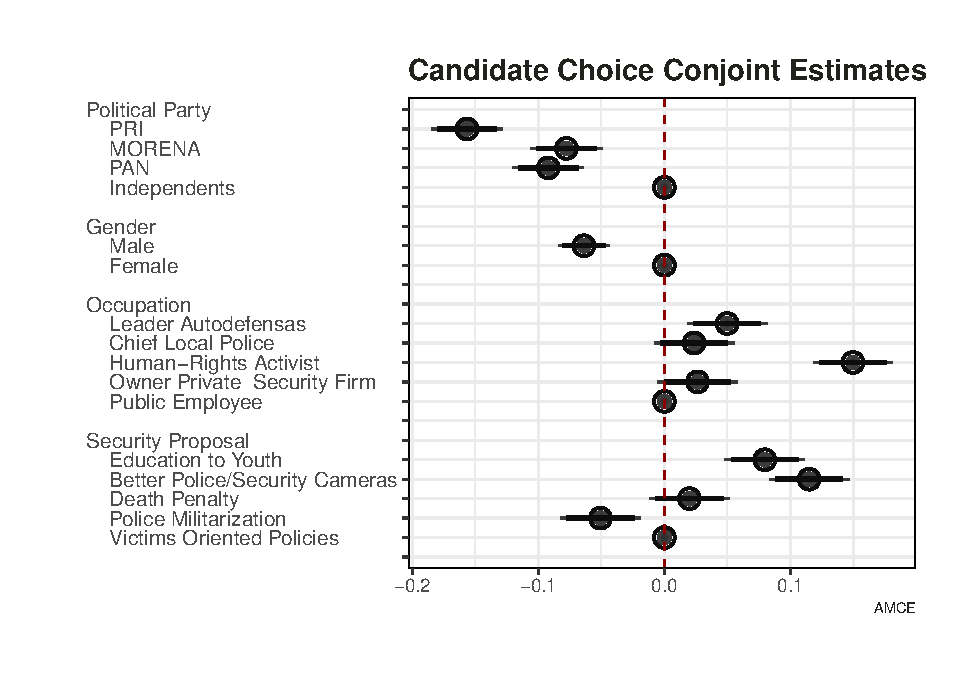
\includegraphics{report_conjoint_candidate_pdf_files/figure-latex/unnamed-chunk-3-1.pdf}

\hypertarget{interaction-effects-party}{%
\subsection{Interaction Effects:
Party}\label{interaction-effects-party}}

\begin{Shaded}
\begin{Highlighting}[]
\NormalTok{conjoint_data <-}\StringTok{ }\NormalTok{conjoint_data }\OperatorTok
\StringTok{                    }\KeywordTok{mutate}\NormalTok{(}\DataTypeTok{vote=}\KeywordTok{ifelse}\NormalTok{(vote_morena}\OperatorTok{==}\StringTok{"On"}\NormalTok{, }\StringTok{"MORENA Voters"}\NormalTok{, }
                                  \KeywordTok{ifelse}\NormalTok{(vote_pri}\OperatorTok{==}\StringTok{"On"}\NormalTok{, }\StringTok{"PRI Voters"}\NormalTok{, }
                                    \KeywordTok{ifelse}\NormalTok{(vote_pan}\OperatorTok{==}\StringTok{"On"}\NormalTok{, }\StringTok{"PAN Voters"}\NormalTok{, }
                                      \StringTok{"Independents"}\NormalTok{))))}

\CommentTok{# By parties}

\NormalTok{res_parties <-}\StringTok{ }\NormalTok{conjoint_data }\OperatorTok\StringTok{ }
\StringTok{                  }\KeywordTok{group_by}\NormalTok{(vote) }\OperatorTok
\StringTok{                  }\KeywordTok{nest}\NormalTok{() }\OperatorTok
\StringTok{                  }\KeywordTok{mutate}\NormalTok{(}\DataTypeTok{model=}\KeywordTok{map2}\NormalTok{(data, vote, }
                                   \OperatorTok{~}\StringTok{ }\KeywordTok{lm}\NormalTok{(outcome_num}\OperatorTok{~}\StringTok{ }\NormalTok{feat_political_party }\OperatorTok{+}\StringTok{ }\NormalTok{feat_gender }\OperatorTok{+}\StringTok{ }
\StringTok{                                          }\NormalTok{feat_security_proposal }\OperatorTok{+}\StringTok{ }\NormalTok{feat_occupation, }
                                          \DataTypeTok{data=}\NormalTok{.x) }\OperatorTok
\StringTok{                                     }\KeywordTok{tidy_conjoint_model}\NormalTok{(}\DataTypeTok{model=}\NormalTok{., }\DataTypeTok{subsample=}\NormalTok{.y, }
                                                         \DataTypeTok{features =}\NormalTok{ features,}
                                     \DataTypeTok{references=}\NormalTok{references, }\DataTypeTok{list_terms =}\NormalTok{ list_terms))) }\OperatorTok\StringTok{ }
\StringTok{                  }\KeywordTok{unnest}\NormalTok{(model)}

\KeywordTok{ggplot}\NormalTok{(res_parties, }\KeywordTok{aes}\NormalTok{(}\DataTypeTok{y=}\NormalTok{estimate, }\DataTypeTok{x=}\NormalTok{term, }
                \DataTypeTok{ymin=}\NormalTok{up, }\DataTypeTok{ymax=}\NormalTok{lb)) }\OperatorTok{+}
\StringTok{  }\KeywordTok{geom_pointrange}\NormalTok{(}\DataTypeTok{size=}\NormalTok{.}\DecValTok{5}\NormalTok{, }\DataTypeTok{fill=}\StringTok{"black"}\NormalTok{, }\DataTypeTok{shape=}\DecValTok{21}\NormalTok{, }\DataTypeTok{color=}\StringTok{"grey5"}\NormalTok{,}
                  \DataTypeTok{position=}\KeywordTok{position_dodge}\NormalTok{(}\DataTypeTok{width =} \FloatTok{.6}\NormalTok{), }\DataTypeTok{alpha=}\NormalTok{.}\DecValTok{8}\NormalTok{) }\OperatorTok{+}
\StringTok{  }\KeywordTok{geom_pointrange}\NormalTok{(}\KeywordTok{aes}\NormalTok{(}\DataTypeTok{ymin=}\NormalTok{lb90, }\DataTypeTok{y=}\NormalTok{estimate, }\DataTypeTok{ymax=}\NormalTok{up90), }\DataTypeTok{shape=}\DecValTok{21}\NormalTok{, }
                  \DataTypeTok{size=}\DecValTok{1}\NormalTok{, }\DataTypeTok{color=}\StringTok{"grey5"}\NormalTok{) }\OperatorTok{+}
\StringTok{  }\KeywordTok{labs}\NormalTok{(}\DataTypeTok{x=}\StringTok{""}\NormalTok{, }\DataTypeTok{y=}\StringTok{"AMCE"}\NormalTok{, }
       \DataTypeTok{title =} \StringTok{"Candidate Choice Conjoint Estimates"}\NormalTok{) }\OperatorTok{+}
\StringTok{  }\KeywordTok{geom_hline}\NormalTok{(}\DataTypeTok{yintercept =} \DecValTok{0}\NormalTok{, }\DataTypeTok{linetype=}\StringTok{"dashed"}\NormalTok{, }\DataTypeTok{color=}\StringTok{"darkred"}\NormalTok{) }\OperatorTok{+}\StringTok{ }
\StringTok{  }\KeywordTok{scale_color_brewer}\NormalTok{(}\DataTypeTok{palette=}\StringTok{"Set1"}\NormalTok{) }\OperatorTok{+}
\StringTok{  }\KeywordTok{coord_flip}\NormalTok{() }\OperatorTok{+}\StringTok{ }
\StringTok{  }\KeywordTok{facet_grid}\NormalTok{(}\OperatorTok{~}\NormalTok{subsample)}\OperatorTok{+}\StringTok{ }
\StringTok{  }\KeywordTok{theme_bw}\NormalTok{()}\OperatorTok{+}\StringTok{ }\NormalTok{my_theme}
\end{Highlighting}
\end{Shaded}

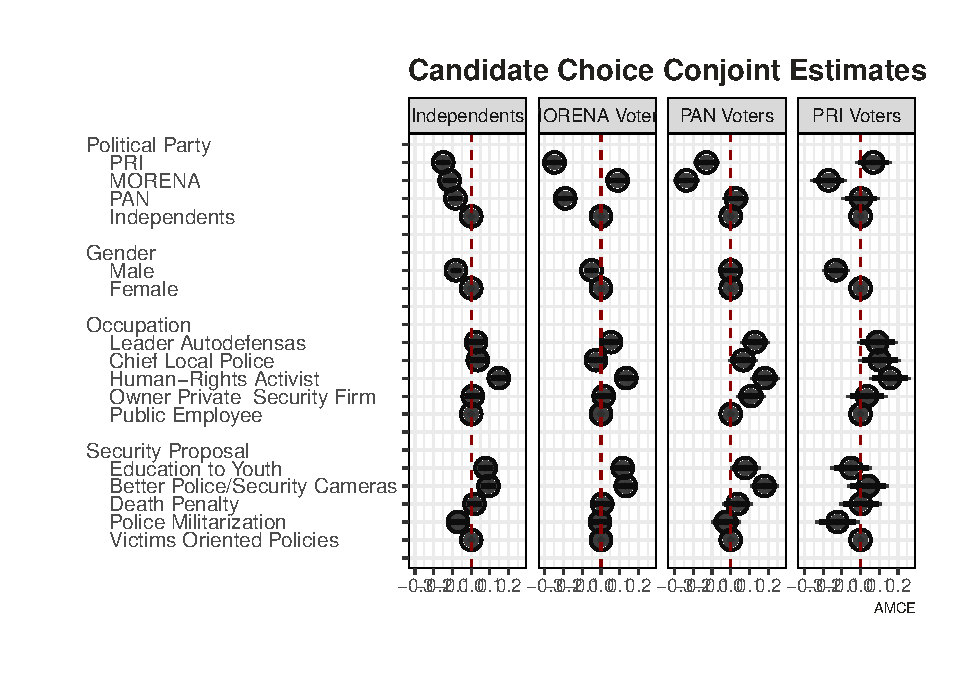
\includegraphics{report_conjoint_candidate_pdf_files/figure-latex/unnamed-chunk-4-1.pdf}

\hypertarget{interaction-effects-crime-victimization}{%
\subsection{Interaction Effects: Crime
Victimization}\label{interaction-effects-crime-victimization}}

\begin{Shaded}
\begin{Highlighting}[]
\CommentTok{# Crime Vitimization ------------------------------------------------------}

\CommentTok{# list levels}

\NormalTok{list_vict <-}\StringTok{ }\KeywordTok{list}\NormalTok{(}\StringTok{"Victim"}\NormalTok{=}\StringTok{ "Si"}\NormalTok{, }
                  \StringTok{"Not Victim"}\NormalTok{ =}\StringTok{ "No"}\NormalTok{)}

\CommentTok{# Recode}
\NormalTok{d_vict <-}\StringTok{ }\NormalTok{conjoint_data }\OperatorTok\StringTok{ }
\StringTok{  }\KeywordTok{mutate_at}\NormalTok{(}\KeywordTok{vars}\NormalTok{(crime_victimization, police_victimization), }\OperatorTok{~}
\StringTok{              }\KeywordTok{ifelse}\NormalTok{(.x }\OperatorTok\StringTok{ }\KeywordTok{c}\NormalTok{(}\StringTok{"-999"}\NormalTok{, }\StringTok{"No lo se"}\NormalTok{), }
                     \OtherTok{NA}\NormalTok{, .x)) }\OperatorTok\StringTok{        }
\StringTok{  }\KeywordTok{mutate_at}\NormalTok{(}\KeywordTok{vars}\NormalTok{(crime_victimization, police_victimization), }\OperatorTok{~}
\StringTok{              }\KeywordTok{fct_recode}\NormalTok{(.x,}\OperatorTok{!!!}\NormalTok{list_vict))}

\NormalTok{d_vict }\OperatorTok\StringTok{ }
\StringTok{  }\KeywordTok{tabyl}\NormalTok{(crime_victimization, police_victimization)}
\end{Highlighting}
\end{Shaded}

\begin{verbatim}
 crime_victimization Not Victim Victim NA_
          Not Victim       6220    474  52
              Victim       1736    542  57
                <NA>         40     14  68
\end{verbatim}

\begin{Shaded}
\begin{Highlighting}[]
\CommentTok{# Model}

\NormalTok{res_vict <-}\StringTok{ }\NormalTok{d_vict }\OperatorTok\StringTok{ }
\StringTok{  }\KeywordTok{group_by}\NormalTok{(crime_victimization) }\OperatorTok\StringTok{ }
\StringTok{  }\KeywordTok{nest}\NormalTok{() }\OperatorTok\StringTok{ }
\StringTok{  }\KeywordTok{drop_na}\NormalTok{() }\OperatorTok
\StringTok{  }\KeywordTok{mutate}\NormalTok{(}\DataTypeTok{model=}\KeywordTok{map2}\NormalTok{(data, crime_victimization, }
                    \OperatorTok{~}\StringTok{ }\KeywordTok{lm}\NormalTok{(outcome_num}\OperatorTok{~}\StringTok{ }\NormalTok{feat_political_party }\OperatorTok{+}\StringTok{ }\NormalTok{feat_gender }\OperatorTok{+}\StringTok{ }
\StringTok{                           }\NormalTok{feat_security_proposal }\OperatorTok{+}\StringTok{ }\NormalTok{feat_occupation, }
                         \DataTypeTok{data=}\NormalTok{.x) }\OperatorTok
\StringTok{                      }\KeywordTok{tidy_conjoint_model}\NormalTok{(}\DataTypeTok{model=}\NormalTok{., }\DataTypeTok{subsample=}\NormalTok{.y, }
                                          \DataTypeTok{features =}\NormalTok{ features,}
                                          \DataTypeTok{references=}\NormalTok{references, }\DataTypeTok{list_terms =}\NormalTok{ list_terms))) }\OperatorTok\StringTok{ }
\StringTok{  }\KeywordTok{unnest}\NormalTok{(model) }\OperatorTok\StringTok{ }\KeywordTok{select}\NormalTok{(}\OperatorTok{-}\NormalTok{data)}



\CommentTok{# Remove repeated}

\NormalTok{res_vict_color <-}\StringTok{ }\NormalTok{res_vict }\OperatorTok\StringTok{ }\KeywordTok{ungroup}\NormalTok{() }\OperatorTok\StringTok{ }
\StringTok{  }\KeywordTok{mutate}\NormalTok{(}\DataTypeTok{id_remove=}\KeywordTok{ifelse}\NormalTok{(crime_victimization}\OperatorTok{==}\StringTok{"Victim"}\OperatorTok{&}\StringTok{ }\NormalTok{(}\KeywordTok{is.na}\NormalTok{(estimate) }\OperatorTok{|}\StringTok{ }\NormalTok{estimate}\OperatorTok{==}\FloatTok{0.0000}\NormalTok{), }\DecValTok{1}\NormalTok{, }\DecValTok{0}\NormalTok{),}
         \DataTypeTok{crime_victimization=}\KeywordTok{fct_rev}\NormalTok{(crime_victimization)) }\OperatorTok
\StringTok{  }\KeywordTok{filter}\NormalTok{(id_remove}\OperatorTok{==}\DecValTok{0}\NormalTok{) }

\KeywordTok{ggplot}\NormalTok{(res_vict_color, }\KeywordTok{aes}\NormalTok{(}\DataTypeTok{y=}\NormalTok{estimate, }\DataTypeTok{x=}\NormalTok{term, }
                        \DataTypeTok{ymin=}\NormalTok{up, }\DataTypeTok{ymax=}\NormalTok{lb, }\DataTypeTok{shape=}\NormalTok{crime_victimization)) }\OperatorTok{+}
\StringTok{  }\KeywordTok{geom_pointrange}\NormalTok{(}\DataTypeTok{size=}\NormalTok{.}\DecValTok{5}\NormalTok{, }\DataTypeTok{fill=}\StringTok{"black"}\NormalTok{, }\DataTypeTok{color=}\StringTok{"grey5"}\NormalTok{,}
                  \DataTypeTok{position=}\KeywordTok{position_dodge}\NormalTok{(}\DataTypeTok{width =} \FloatTok{.6}\NormalTok{), }\DataTypeTok{alpha=}\NormalTok{.}\DecValTok{8}\NormalTok{) }\OperatorTok{+}
\StringTok{  }\KeywordTok{labs}\NormalTok{(}\DataTypeTok{x=}\StringTok{""}\NormalTok{, }\DataTypeTok{y=}\StringTok{"AMCE"}\NormalTok{, }
       \DataTypeTok{title =} \StringTok{"Candidate Choice Conjoint Estimates"}\NormalTok{) }\OperatorTok{+}
\StringTok{  }\KeywordTok{geom_hline}\NormalTok{(}\DataTypeTok{yintercept =} \DecValTok{0}\NormalTok{, }\DataTypeTok{linetype=}\StringTok{"dashed"}\NormalTok{, }\DataTypeTok{color=}\StringTok{"darkred"}\NormalTok{) }\OperatorTok{+}\StringTok{ }
\StringTok{  }\KeywordTok{scale_shape_manual}\NormalTok{(}\DataTypeTok{values=}\KeywordTok{c}\NormalTok{(}\DecValTok{22}\NormalTok{,}\DecValTok{23}\NormalTok{), }\DataTypeTok{name=}\StringTok{"Crime Victimization"}\NormalTok{) }\OperatorTok{+}
\StringTok{  }\KeywordTok{coord_flip}\NormalTok{() }\OperatorTok{+}\StringTok{ }
\StringTok{  }\KeywordTok{theme_bw}\NormalTok{()}\OperatorTok{+}\StringTok{ }\NormalTok{my_theme}
\end{Highlighting}
\end{Shaded}

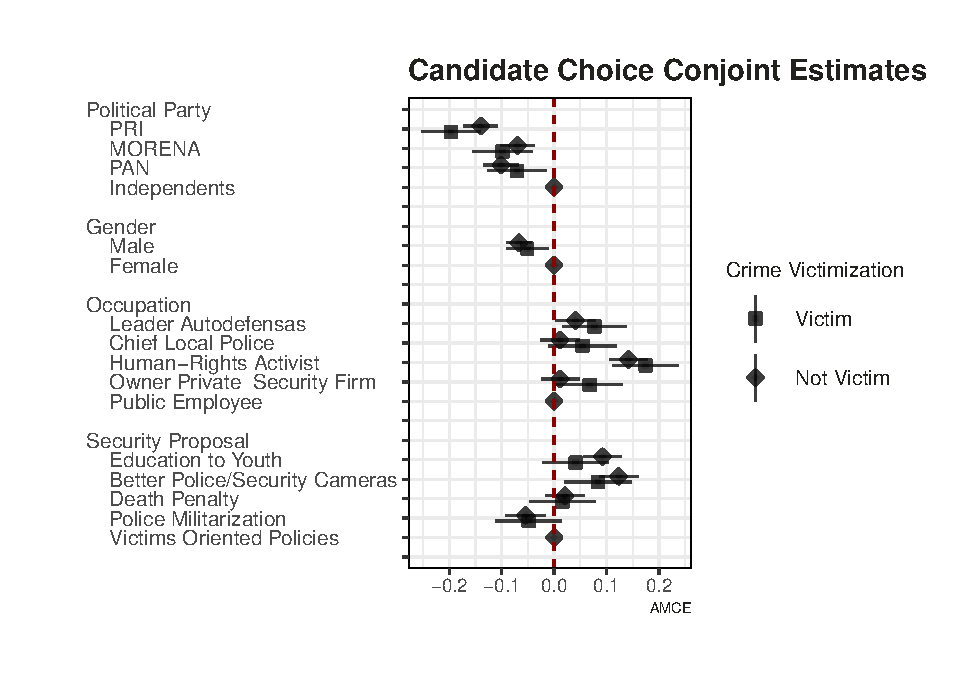
\includegraphics{report_conjoint_candidate_pdf_files/figure-latex/unnamed-chunk-5-1.pdf}

\hypertarget{interaction-effects-police-victimization}{%
\subsection{Interaction Effects: Police
Victimization}\label{interaction-effects-police-victimization}}

\begin{Shaded}
\begin{Highlighting}[]
\CommentTok{# Model}

\NormalTok{res_vict <-}\StringTok{ }\NormalTok{d_vict }\OperatorTok\StringTok{ }
\StringTok{  }\KeywordTok{group_by}\NormalTok{(police_victimization) }\OperatorTok\StringTok{ }
\StringTok{  }\KeywordTok{nest}\NormalTok{() }\OperatorTok\StringTok{ }
\StringTok{  }\KeywordTok{drop_na}\NormalTok{() }\OperatorTok
\StringTok{  }\KeywordTok{mutate}\NormalTok{(}\DataTypeTok{model=}\KeywordTok{map2}\NormalTok{(data, police_victimization, }
                    \OperatorTok{~}\StringTok{ }\KeywordTok{lm}\NormalTok{(outcome_num}\OperatorTok{~}\StringTok{ }\NormalTok{feat_political_party }\OperatorTok{+}\StringTok{ }\NormalTok{feat_gender }\OperatorTok{+}\StringTok{ }
\StringTok{                           }\NormalTok{feat_security_proposal }\OperatorTok{+}\StringTok{ }\NormalTok{feat_occupation, }
                         \DataTypeTok{data=}\NormalTok{.x) }\OperatorTok
\StringTok{                      }\KeywordTok{tidy_conjoint_model}\NormalTok{(}\DataTypeTok{model=}\NormalTok{., }\DataTypeTok{subsample=}\NormalTok{.y, }
                                          \DataTypeTok{features =}\NormalTok{ features,}
                                          \DataTypeTok{references=}\NormalTok{references, }\DataTypeTok{list_terms =}\NormalTok{ list_terms))) }\OperatorTok\StringTok{ }
\StringTok{  }\KeywordTok{unnest}\NormalTok{(model) }\OperatorTok\StringTok{ }\KeywordTok{select}\NormalTok{(}\OperatorTok{-}\NormalTok{data)}



\CommentTok{# Remove repeated}

\NormalTok{res_vict_color <-}\StringTok{ }\NormalTok{res_vict }\OperatorTok\StringTok{ }\KeywordTok{ungroup}\NormalTok{() }\OperatorTok\StringTok{ }
\StringTok{  }\KeywordTok{mutate}\NormalTok{(}\DataTypeTok{id_remove=}\KeywordTok{ifelse}\NormalTok{(police_victimization}\OperatorTok{==}\StringTok{"Victim"}\OperatorTok{&}\StringTok{ }\NormalTok{(}\KeywordTok{is.na}\NormalTok{(estimate) }\OperatorTok{|}\StringTok{ }\NormalTok{estimate}\OperatorTok{==}\FloatTok{0.0000}\NormalTok{), }\DecValTok{1}\NormalTok{, }\DecValTok{0}\NormalTok{)) }\OperatorTok
\StringTok{  }\KeywordTok{filter}\NormalTok{(id_remove}\OperatorTok{==}\DecValTok{0}\NormalTok{) }

\NormalTok{res_vict_color }\OperatorTok\StringTok{ }\KeywordTok{View}\NormalTok{()}

\KeywordTok{ggplot}\NormalTok{(res_vict_color, }\KeywordTok{aes}\NormalTok{(}\DataTypeTok{y=}\NormalTok{estimate, }\DataTypeTok{x=}\NormalTok{term, }
                           \DataTypeTok{ymin=}\NormalTok{up, }\DataTypeTok{ymax=}\NormalTok{lb, }\DataTypeTok{shape=}\NormalTok{police_victimization)) }\OperatorTok{+}
\StringTok{  }\KeywordTok{geom_pointrange}\NormalTok{(}\DataTypeTok{size=}\NormalTok{.}\DecValTok{5}\NormalTok{, }\DataTypeTok{fill=}\StringTok{"black"}\NormalTok{, }\DataTypeTok{color=}\StringTok{"grey5"}\NormalTok{,}
                  \DataTypeTok{position=}\KeywordTok{position_dodge}\NormalTok{(}\DataTypeTok{width =} \FloatTok{.7}\NormalTok{), }\DataTypeTok{alpha=}\NormalTok{.}\DecValTok{8}\NormalTok{) }\OperatorTok{+}
\StringTok{  }\KeywordTok{labs}\NormalTok{(}\DataTypeTok{x=}\StringTok{""}\NormalTok{, }\DataTypeTok{y=}\StringTok{"AMCE"}\NormalTok{, }
       \DataTypeTok{title =} \StringTok{"Candidate Choice Conjoint Estimates"}\NormalTok{) }\OperatorTok{+}
\StringTok{  }\KeywordTok{geom_hline}\NormalTok{(}\DataTypeTok{yintercept =} \DecValTok{0}\NormalTok{, }\DataTypeTok{linetype=}\StringTok{"dashed"}\NormalTok{, }\DataTypeTok{color=}\StringTok{"darkred"}\NormalTok{) }\OperatorTok{+}\StringTok{ }
\StringTok{  }\KeywordTok{scale_shape_manual}\NormalTok{(}\DataTypeTok{values=}\KeywordTok{c}\NormalTok{(}\DecValTok{22}\NormalTok{,}\DecValTok{23}\NormalTok{), }\DataTypeTok{name=}\StringTok{"Police Victimization"}\NormalTok{) }\OperatorTok{+}
\StringTok{  }\KeywordTok{coord_flip}\NormalTok{() }\OperatorTok{+}\StringTok{ }
\StringTok{  }\KeywordTok{guides}\NormalTok{(}\DataTypeTok{shape =} \KeywordTok{guide_legend}\NormalTok{(}\DataTypeTok{reverse=}\NormalTok{T)) }\OperatorTok{+}
\StringTok{  }\KeywordTok{theme_bw}\NormalTok{()}\OperatorTok{+}\StringTok{ }\NormalTok{my_theme}
\end{Highlighting}
\end{Shaded}

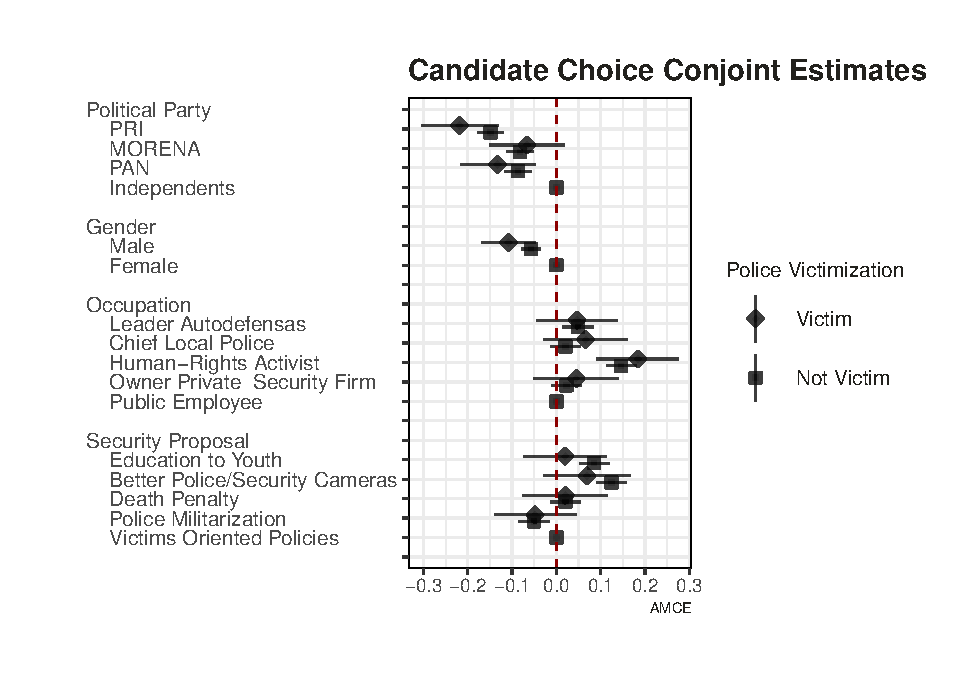
\includegraphics{report_conjoint_candidate_pdf_files/figure-latex/unnamed-chunk-6-1.pdf}

\hypertarget{fear-of-crime}{%
\subsection{Fear of Crime}\label{fear-of-crime}}

\begin{Shaded}
\begin{Highlighting}[]
\CommentTok{# Fear of Crime -----------------------------------------------------------}


\CommentTok{# list levels}

\CommentTok{# Recode}
\NormalTok{d_fear <-}\StringTok{ }\NormalTok{conjoint_data }\OperatorTok\StringTok{ }
\StringTok{  }\KeywordTok{mutate_at}\NormalTok{(}\KeywordTok{vars}\NormalTok{(fear_}\DecValTok{1}\NormalTok{, fear_}\DecValTok{2}\NormalTok{, fear_}\DecValTok{3}\NormalTok{, fear_}\DecValTok{4}\NormalTok{), }\OperatorTok{~}\StringTok{ }
\StringTok{              }\KeywordTok{ifelse}\NormalTok{(.x }\OperatorTok\StringTok{ }\KeywordTok{c}\NormalTok{(}\StringTok{"-999"}\NormalTok{, }\StringTok{"No lo se"}\NormalTok{), }
                     \OtherTok{NA}\NormalTok{, .x)) }\OperatorTok
\StringTok{  }\KeywordTok{mutate_at}\NormalTok{(}\KeywordTok{vars}\NormalTok{(fear_}\DecValTok{1}\NormalTok{, fear_}\DecValTok{2}\NormalTok{, fear_}\DecValTok{3}\NormalTok{, fear_}\DecValTok{4}\NormalTok{), }\OperatorTok{~}\StringTok{ }
\StringTok{              }\KeywordTok{fct_relevel}\NormalTok{(.x, }\StringTok{"Muy Seguro"}\NormalTok{, }\StringTok{"Seguro"}\NormalTok{, }\StringTok{"Poco Seguro"}\NormalTok{))}

\CommentTok{# Model}
\NormalTok{res_fear <-}\StringTok{ }\NormalTok{d_fear }\OperatorTok\StringTok{ }
\StringTok{  }\KeywordTok{group_by}\NormalTok{(fear_}\DecValTok{1}\NormalTok{) }\OperatorTok\StringTok{ }
\StringTok{  }\KeywordTok{nest}\NormalTok{() }\OperatorTok\StringTok{ }
\StringTok{  }\KeywordTok{drop_na}\NormalTok{() }\OperatorTok
\StringTok{  }\KeywordTok{mutate}\NormalTok{(}\DataTypeTok{model=}\KeywordTok{map2}\NormalTok{(data, fear_}\DecValTok{1}\NormalTok{, }
                    \OperatorTok{~}\StringTok{ }\KeywordTok{lm}\NormalTok{(outcome_num}\OperatorTok{~}\StringTok{ }\NormalTok{feat_political_party }\OperatorTok{+}\StringTok{ }\NormalTok{feat_gender }\OperatorTok{+}\StringTok{ }
\StringTok{                           }\NormalTok{feat_security_proposal }\OperatorTok{+}\StringTok{ }\NormalTok{feat_occupation, }
                         \DataTypeTok{data=}\NormalTok{.x) }\OperatorTok
\StringTok{                      }\KeywordTok{tidy_conjoint_model}\NormalTok{(}\DataTypeTok{model=}\NormalTok{., }\DataTypeTok{subsample=}\NormalTok{.y, }
                                          \DataTypeTok{features =}\NormalTok{ features,}
                                          \DataTypeTok{references=}\NormalTok{references, }\DataTypeTok{list_terms =}\NormalTok{ list_terms))) }\OperatorTok\StringTok{ }
\StringTok{  }\KeywordTok{unnest}\NormalTok{(model) }\OperatorTok\StringTok{ }\KeywordTok{select}\NormalTok{(}\OperatorTok{-}\NormalTok{data)}



\CommentTok{# # Remove repeated}
\CommentTok{# }
\CommentTok{# res_vict_color <- res_vict %>% ungroup() %>% }
\CommentTok{#   mutate(id_remove=ifelse(crime_victimization=="Victim"& (is.na(estimate) | estimate==0.0000), 1, 0),}
\CommentTok{#          crime_victimization=fct_rev(crime_victimization)) %>%}
\CommentTok{#   filter(id_remove==0) }


\KeywordTok{ggplot}\NormalTok{(res_fear, }\KeywordTok{aes}\NormalTok{(}\DataTypeTok{y=}\NormalTok{estimate, }\DataTypeTok{x=}\NormalTok{term, }
                        \DataTypeTok{ymin=}\NormalTok{up, }\DataTypeTok{ymax=}\NormalTok{lb)) }\OperatorTok{+}
\StringTok{  }\KeywordTok{geom_pointrange}\NormalTok{(}\DataTypeTok{size=}\NormalTok{.}\DecValTok{5}\NormalTok{, }\DataTypeTok{fill=}\StringTok{"black"}\NormalTok{, }\DataTypeTok{shape=}\DecValTok{21}\NormalTok{, }\DataTypeTok{color=}\StringTok{"grey5"}\NormalTok{,}
                  \DataTypeTok{position=}\KeywordTok{position_dodge}\NormalTok{(}\DataTypeTok{width =} \FloatTok{.6}\NormalTok{), }\DataTypeTok{alpha=}\NormalTok{.}\DecValTok{8}\NormalTok{) }\OperatorTok{+}
\StringTok{  }\KeywordTok{geom_pointrange}\NormalTok{(}\KeywordTok{aes}\NormalTok{(}\DataTypeTok{ymin=}\NormalTok{lb90, }\DataTypeTok{y=}\NormalTok{estimate, }\DataTypeTok{ymax=}\NormalTok{up90), }\DataTypeTok{shape=}\DecValTok{21}\NormalTok{, }
                  \DataTypeTok{size=}\DecValTok{1}\NormalTok{, }\DataTypeTok{color=}\StringTok{"grey5"}\NormalTok{) }\OperatorTok{+}
\StringTok{  }\KeywordTok{labs}\NormalTok{(}\DataTypeTok{x=}\StringTok{""}\NormalTok{, }\DataTypeTok{y=}\StringTok{"AMCE"}\NormalTok{, }
       \DataTypeTok{title =} \StringTok{"Candidate Choice Conjoint Estimates"}\NormalTok{, }
       \DataTypeTok{subtitle =} \StringTok{"Fear: Caminando solo(a) en una calle oscura"}\NormalTok{) }\OperatorTok{+}
\StringTok{  }\KeywordTok{geom_hline}\NormalTok{(}\DataTypeTok{yintercept =} \DecValTok{0}\NormalTok{, }\DataTypeTok{linetype=}\StringTok{"dashed"}\NormalTok{, }\DataTypeTok{color=}\StringTok{"darkred"}\NormalTok{) }\OperatorTok{+}\StringTok{ }
\StringTok{  }\KeywordTok{scale_color_brewer}\NormalTok{(}\DataTypeTok{palette=}\StringTok{"Set1"}\NormalTok{) }\OperatorTok{+}
\StringTok{  }\KeywordTok{coord_flip}\NormalTok{() }\OperatorTok{+}\StringTok{ }
\StringTok{  }\KeywordTok{facet_grid}\NormalTok{(}\OperatorTok{~}\NormalTok{subsample) }\OperatorTok{+}\StringTok{ }
\StringTok{  }\KeywordTok{theme_bw}\NormalTok{()}\OperatorTok{+}\StringTok{ }\NormalTok{my_theme}
\end{Highlighting}
\end{Shaded}

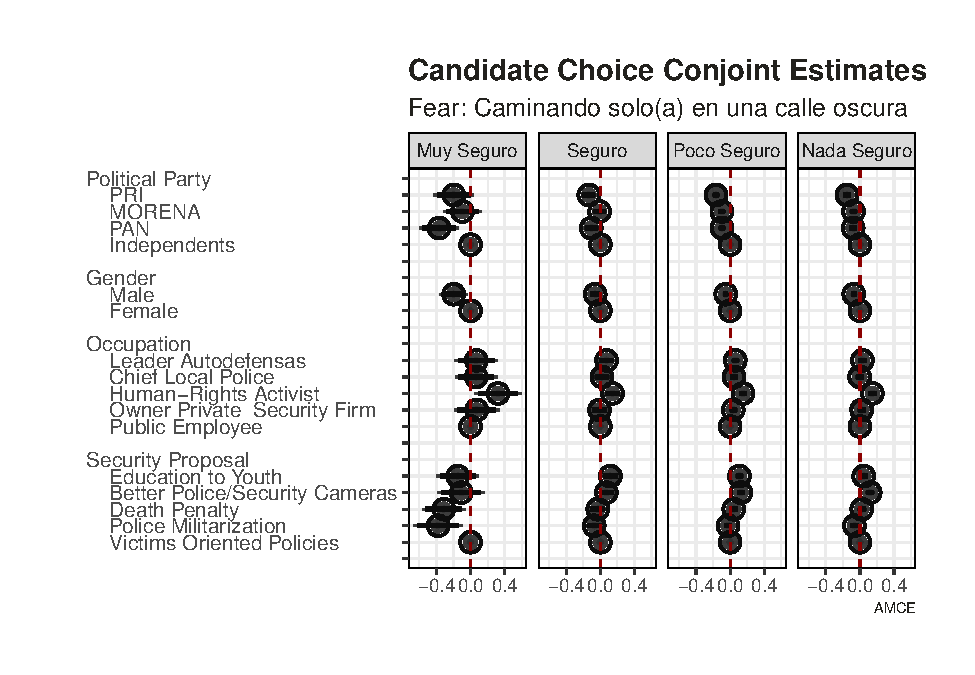
\includegraphics{report_conjoint_candidate_pdf_files/figure-latex/unnamed-chunk-7-1.pdf}

\begin{Shaded}
\begin{Highlighting}[]
\CommentTok{# Fear 2}

\CommentTok{# Model}
\NormalTok{res_fear <-}\StringTok{ }\NormalTok{d_fear }\OperatorTok\StringTok{ }
\StringTok{  }\KeywordTok{group_by}\NormalTok{(fear_}\DecValTok{2}\NormalTok{) }\OperatorTok\StringTok{ }
\StringTok{  }\KeywordTok{nest}\NormalTok{() }\OperatorTok\StringTok{ }
\StringTok{  }\KeywordTok{drop_na}\NormalTok{() }\OperatorTok
\StringTok{  }\KeywordTok{mutate}\NormalTok{(}\DataTypeTok{model=}\KeywordTok{map2}\NormalTok{(data, fear_}\DecValTok{2}\NormalTok{, }
                    \OperatorTok{~}\StringTok{ }\KeywordTok{lm}\NormalTok{(outcome_num}\OperatorTok{~}\StringTok{ }\NormalTok{feat_political_party }\OperatorTok{+}\StringTok{ }\NormalTok{feat_gender }\OperatorTok{+}\StringTok{ }
\StringTok{                           }\NormalTok{feat_security_proposal }\OperatorTok{+}\StringTok{ }\NormalTok{feat_occupation, }
                         \DataTypeTok{data=}\NormalTok{.x) }\OperatorTok
\StringTok{                      }\KeywordTok{tidy_conjoint_model}\NormalTok{(}\DataTypeTok{model=}\NormalTok{., }\DataTypeTok{subsample=}\NormalTok{.y, }
                                          \DataTypeTok{features =}\NormalTok{ features,}
                                          \DataTypeTok{references=}\NormalTok{references, }\DataTypeTok{list_terms =}\NormalTok{ list_terms))) }\OperatorTok\StringTok{ }
\StringTok{  }\KeywordTok{unnest}\NormalTok{(model) }\OperatorTok\StringTok{ }\KeywordTok{select}\NormalTok{(}\OperatorTok{-}\NormalTok{data)}


\KeywordTok{ggplot}\NormalTok{(res_fear, }\KeywordTok{aes}\NormalTok{(}\DataTypeTok{y=}\NormalTok{estimate, }\DataTypeTok{x=}\NormalTok{term, }
                     \DataTypeTok{ymin=}\NormalTok{up, }\DataTypeTok{ymax=}\NormalTok{lb)) }\OperatorTok{+}
\StringTok{  }\KeywordTok{geom_pointrange}\NormalTok{(}\DataTypeTok{size=}\NormalTok{.}\DecValTok{5}\NormalTok{, }\DataTypeTok{fill=}\StringTok{"black"}\NormalTok{, }\DataTypeTok{shape=}\DecValTok{21}\NormalTok{, }\DataTypeTok{color=}\StringTok{"grey5"}\NormalTok{,}
                  \DataTypeTok{position=}\KeywordTok{position_dodge}\NormalTok{(}\DataTypeTok{width =} \FloatTok{.6}\NormalTok{), }\DataTypeTok{alpha=}\NormalTok{.}\DecValTok{8}\NormalTok{) }\OperatorTok{+}
\StringTok{  }\KeywordTok{geom_pointrange}\NormalTok{(}\KeywordTok{aes}\NormalTok{(}\DataTypeTok{ymin=}\NormalTok{lb90, }\DataTypeTok{y=}\NormalTok{estimate, }\DataTypeTok{ymax=}\NormalTok{up90), }\DataTypeTok{shape=}\DecValTok{21}\NormalTok{, }
                  \DataTypeTok{size=}\DecValTok{1}\NormalTok{, }\DataTypeTok{color=}\StringTok{"grey5"}\NormalTok{) }\OperatorTok{+}
\StringTok{  }\KeywordTok{labs}\NormalTok{(}\DataTypeTok{x=}\StringTok{""}\NormalTok{, }\DataTypeTok{y=}\StringTok{"AMCE"}\NormalTok{, }
       \DataTypeTok{title =} \StringTok{"Candidate Choice Conjoint Estimates"}\NormalTok{, }
       \DataTypeTok{subtitle =} \StringTok{"Fear: Conducir en tu ciudad durante la noche"}\NormalTok{) }\OperatorTok{+}
\StringTok{  }\KeywordTok{geom_hline}\NormalTok{(}\DataTypeTok{yintercept =} \DecValTok{0}\NormalTok{, }\DataTypeTok{linetype=}\StringTok{"dashed"}\NormalTok{, }\DataTypeTok{color=}\StringTok{"darkred"}\NormalTok{) }\OperatorTok{+}\StringTok{ }
\StringTok{  }\KeywordTok{scale_color_brewer}\NormalTok{(}\DataTypeTok{palette=}\StringTok{"Set1"}\NormalTok{) }\OperatorTok{+}
\StringTok{  }\KeywordTok{coord_flip}\NormalTok{() }\OperatorTok{+}\StringTok{ }
\StringTok{  }\KeywordTok{facet_grid}\NormalTok{(}\OperatorTok{~}\NormalTok{subsample) }\OperatorTok{+}\StringTok{ }
\StringTok{  }\KeywordTok{theme_bw}\NormalTok{()}\OperatorTok{+}\StringTok{ }\NormalTok{my_theme}
\end{Highlighting}
\end{Shaded}

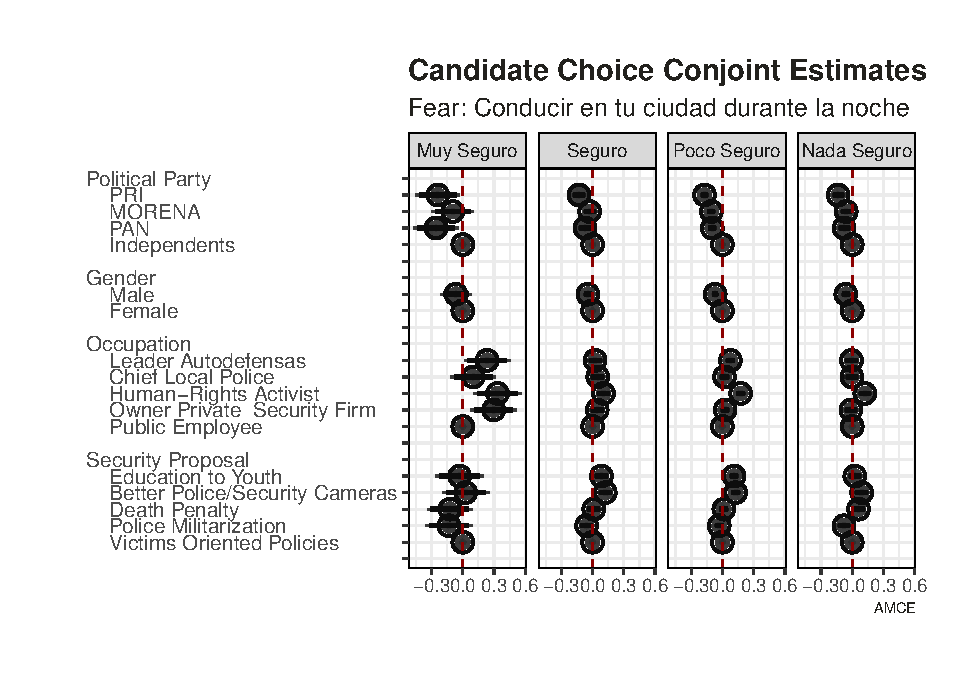
\includegraphics{report_conjoint_candidate_pdf_files/figure-latex/unnamed-chunk-7-2.pdf}

\begin{Shaded}
\begin{Highlighting}[]
\CommentTok{# Fear 3}

\CommentTok{# Model}
\NormalTok{res_fear <-}\StringTok{ }\NormalTok{d_fear }\OperatorTok\StringTok{ }
\StringTok{  }\KeywordTok{group_by}\NormalTok{(fear_}\DecValTok{3}\NormalTok{) }\OperatorTok\StringTok{ }
\StringTok{  }\KeywordTok{nest}\NormalTok{() }\OperatorTok\StringTok{ }
\StringTok{  }\KeywordTok{drop_na}\NormalTok{() }\OperatorTok
\StringTok{  }\KeywordTok{mutate}\NormalTok{(}\DataTypeTok{model=}\KeywordTok{map2}\NormalTok{(data, fear_}\DecValTok{3}\NormalTok{, }
                    \OperatorTok{~}\StringTok{ }\KeywordTok{lm}\NormalTok{(outcome_num}\OperatorTok{~}\StringTok{ }\NormalTok{feat_political_party }\OperatorTok{+}\StringTok{ }\NormalTok{feat_gender }\OperatorTok{+}\StringTok{ }
\StringTok{                           }\NormalTok{feat_security_proposal }\OperatorTok{+}\StringTok{ }\NormalTok{feat_occupation, }
                         \DataTypeTok{data=}\NormalTok{.x) }\OperatorTok
\StringTok{                      }\KeywordTok{tidy_conjoint_model}\NormalTok{(}\DataTypeTok{model=}\NormalTok{., }\DataTypeTok{subsample=}\NormalTok{.y, }
                                          \DataTypeTok{features =}\NormalTok{ features,}
                                          \DataTypeTok{references=}\NormalTok{references, }\DataTypeTok{list_terms =}\NormalTok{ list_terms))) }\OperatorTok\StringTok{ }
\StringTok{  }\KeywordTok{unnest}\NormalTok{(model) }\OperatorTok\StringTok{ }\KeywordTok{select}\NormalTok{(}\OperatorTok{-}\NormalTok{data)}


\KeywordTok{ggplot}\NormalTok{(res_fear, }\KeywordTok{aes}\NormalTok{(}\DataTypeTok{y=}\NormalTok{estimate, }\DataTypeTok{x=}\NormalTok{term, }
                     \DataTypeTok{ymin=}\NormalTok{up, }\DataTypeTok{ymax=}\NormalTok{lb)) }\OperatorTok{+}
\StringTok{  }\KeywordTok{geom_pointrange}\NormalTok{(}\DataTypeTok{size=}\NormalTok{.}\DecValTok{5}\NormalTok{, }\DataTypeTok{fill=}\StringTok{"black"}\NormalTok{, }\DataTypeTok{shape=}\DecValTok{21}\NormalTok{, }\DataTypeTok{color=}\StringTok{"grey5"}\NormalTok{,}
                  \DataTypeTok{position=}\KeywordTok{position_dodge}\NormalTok{(}\DataTypeTok{width =} \FloatTok{.6}\NormalTok{), }\DataTypeTok{alpha=}\NormalTok{.}\DecValTok{8}\NormalTok{) }\OperatorTok{+}
\StringTok{  }\KeywordTok{geom_pointrange}\NormalTok{(}\KeywordTok{aes}\NormalTok{(}\DataTypeTok{ymin=}\NormalTok{lb90, }\DataTypeTok{y=}\NormalTok{estimate, }\DataTypeTok{ymax=}\NormalTok{up90), }\DataTypeTok{shape=}\DecValTok{21}\NormalTok{, }
                  \DataTypeTok{size=}\DecValTok{1}\NormalTok{, }\DataTypeTok{color=}\StringTok{"grey5"}\NormalTok{) }\OperatorTok{+}
\StringTok{  }\KeywordTok{labs}\NormalTok{(}\DataTypeTok{x=}\StringTok{""}\NormalTok{, }\DataTypeTok{y=}\StringTok{"AMCE"}\NormalTok{, }
       \DataTypeTok{title =} \StringTok{"Candidate Choice Conjoint Estimates"}\NormalTok{, }
       \DataTypeTok{subtitle =} \StringTok{"Fear: Quedarse solo en casa"}\NormalTok{) }\OperatorTok{+}
\StringTok{  }\KeywordTok{geom_hline}\NormalTok{(}\DataTypeTok{yintercept =} \DecValTok{0}\NormalTok{, }\DataTypeTok{linetype=}\StringTok{"dashed"}\NormalTok{, }\DataTypeTok{color=}\StringTok{"darkred"}\NormalTok{) }\OperatorTok{+}\StringTok{ }
\StringTok{  }\KeywordTok{scale_color_brewer}\NormalTok{(}\DataTypeTok{palette=}\StringTok{"Set1"}\NormalTok{) }\OperatorTok{+}
\StringTok{  }\KeywordTok{coord_flip}\NormalTok{() }\OperatorTok{+}\StringTok{ }
\StringTok{  }\KeywordTok{facet_grid}\NormalTok{(}\OperatorTok{~}\NormalTok{subsample) }\OperatorTok{+}\StringTok{ }
\StringTok{  }\KeywordTok{theme_bw}\NormalTok{()}\OperatorTok{+}\StringTok{ }\NormalTok{my_theme}
\end{Highlighting}
\end{Shaded}

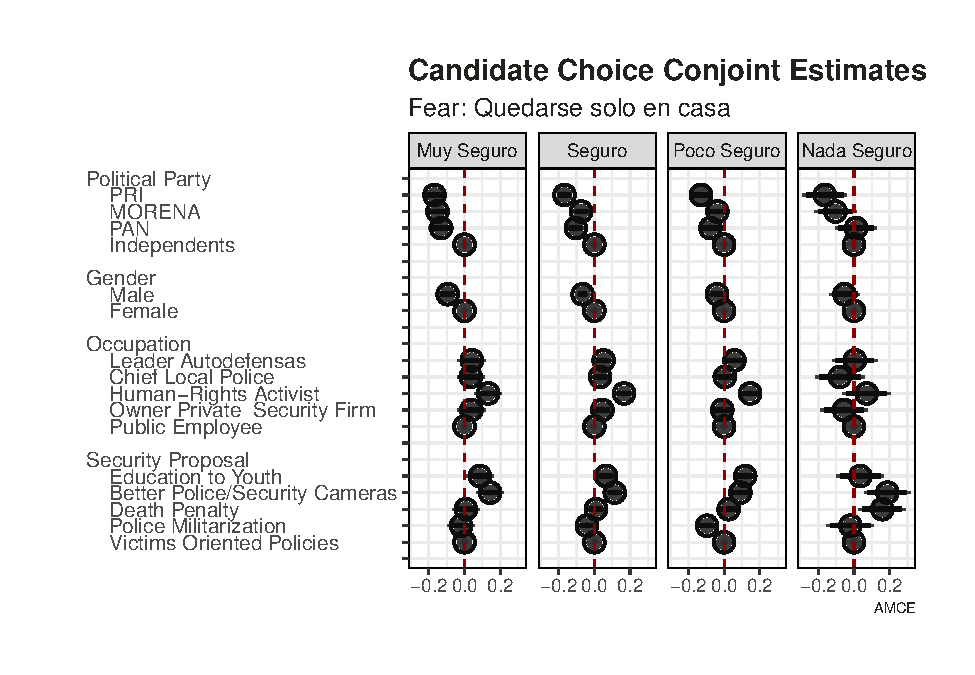
\includegraphics{report_conjoint_candidate_pdf_files/figure-latex/unnamed-chunk-7-3.pdf}

\begin{Shaded}
\begin{Highlighting}[]
\CommentTok{# Fear 4}

\CommentTok{# Model}
\NormalTok{res_fear <-}\StringTok{ }\NormalTok{d_fear }\OperatorTok\StringTok{ }
\StringTok{  }\KeywordTok{group_by}\NormalTok{(fear_}\DecValTok{4}\NormalTok{) }\OperatorTok\StringTok{ }
\StringTok{  }\KeywordTok{nest}\NormalTok{() }\OperatorTok\StringTok{ }
\StringTok{  }\KeywordTok{drop_na}\NormalTok{() }\OperatorTok
\StringTok{  }\KeywordTok{mutate}\NormalTok{(}\DataTypeTok{model=}\KeywordTok{map2}\NormalTok{(data, fear_}\DecValTok{4}\NormalTok{, }
                    \OperatorTok{~}\StringTok{ }\KeywordTok{lm}\NormalTok{(outcome_num}\OperatorTok{~}\StringTok{ }\NormalTok{feat_political_party }\OperatorTok{+}\StringTok{ }\NormalTok{feat_gender }\OperatorTok{+}\StringTok{ }
\StringTok{                           }\NormalTok{feat_security_proposal }\OperatorTok{+}\StringTok{ }\NormalTok{feat_occupation, }
                         \DataTypeTok{data=}\NormalTok{.x) }\OperatorTok
\StringTok{                      }\KeywordTok{tidy_conjoint_model}\NormalTok{(}\DataTypeTok{model=}\NormalTok{., }\DataTypeTok{subsample=}\NormalTok{.y, }
                                          \DataTypeTok{features =}\NormalTok{ features,}
                                          \DataTypeTok{references=}\NormalTok{references, }\DataTypeTok{list_terms =}\NormalTok{ list_terms))) }\OperatorTok\StringTok{ }
\StringTok{  }\KeywordTok{unnest}\NormalTok{(model) }\OperatorTok\StringTok{ }\KeywordTok{select}\NormalTok{(}\OperatorTok{-}\NormalTok{data)}


\KeywordTok{ggplot}\NormalTok{(res_fear, }\KeywordTok{aes}\NormalTok{(}\DataTypeTok{y=}\NormalTok{estimate, }\DataTypeTok{x=}\NormalTok{term, }
                     \DataTypeTok{ymin=}\NormalTok{up, }\DataTypeTok{ymax=}\NormalTok{lb)) }\OperatorTok{+}
\StringTok{  }\KeywordTok{geom_pointrange}\NormalTok{(}\DataTypeTok{size=}\NormalTok{.}\DecValTok{5}\NormalTok{, }\DataTypeTok{fill=}\StringTok{"black"}\NormalTok{, }\DataTypeTok{shape=}\DecValTok{21}\NormalTok{, }\DataTypeTok{color=}\StringTok{"grey5"}\NormalTok{,}
                  \DataTypeTok{position=}\KeywordTok{position_dodge}\NormalTok{(}\DataTypeTok{width =} \FloatTok{.6}\NormalTok{), }\DataTypeTok{alpha=}\NormalTok{.}\DecValTok{8}\NormalTok{) }\OperatorTok{+}
\StringTok{  }\KeywordTok{geom_pointrange}\NormalTok{(}\KeywordTok{aes}\NormalTok{(}\DataTypeTok{ymin=}\NormalTok{lb90, }\DataTypeTok{y=}\NormalTok{estimate, }\DataTypeTok{ymax=}\NormalTok{up90), }\DataTypeTok{shape=}\DecValTok{21}\NormalTok{, }
                  \DataTypeTok{size=}\DecValTok{1}\NormalTok{, }\DataTypeTok{color=}\StringTok{"grey5"}\NormalTok{) }\OperatorTok{+}
\StringTok{  }\KeywordTok{labs}\NormalTok{(}\DataTypeTok{x=}\StringTok{""}\NormalTok{, }\DataTypeTok{y=}\StringTok{"AMCE"}\NormalTok{, }
       \DataTypeTok{title =} \StringTok{"Candidate Choice Conjoint Estimates"}\NormalTok{, }
       \DataTypeTok{subtitle =} \StringTok{"Fear: Al encontrar una patrulla policial en su vecindario"}\NormalTok{) }\OperatorTok{+}
\StringTok{  }\KeywordTok{geom_hline}\NormalTok{(}\DataTypeTok{yintercept =} \DecValTok{0}\NormalTok{, }\DataTypeTok{linetype=}\StringTok{"dashed"}\NormalTok{, }\DataTypeTok{color=}\StringTok{"darkred"}\NormalTok{) }\OperatorTok{+}\StringTok{ }
\StringTok{  }\KeywordTok{scale_color_brewer}\NormalTok{(}\DataTypeTok{palette=}\StringTok{"Set1"}\NormalTok{) }\OperatorTok{+}
\StringTok{  }\KeywordTok{coord_flip}\NormalTok{() }\OperatorTok{+}\StringTok{ }
\StringTok{  }\KeywordTok{facet_grid}\NormalTok{(}\OperatorTok{~}\NormalTok{subsample) }\OperatorTok{+}\StringTok{ }
\StringTok{  }\KeywordTok{theme_bw}\NormalTok{()}\OperatorTok{+}\StringTok{ }\NormalTok{my_theme}
\end{Highlighting}
\end{Shaded}

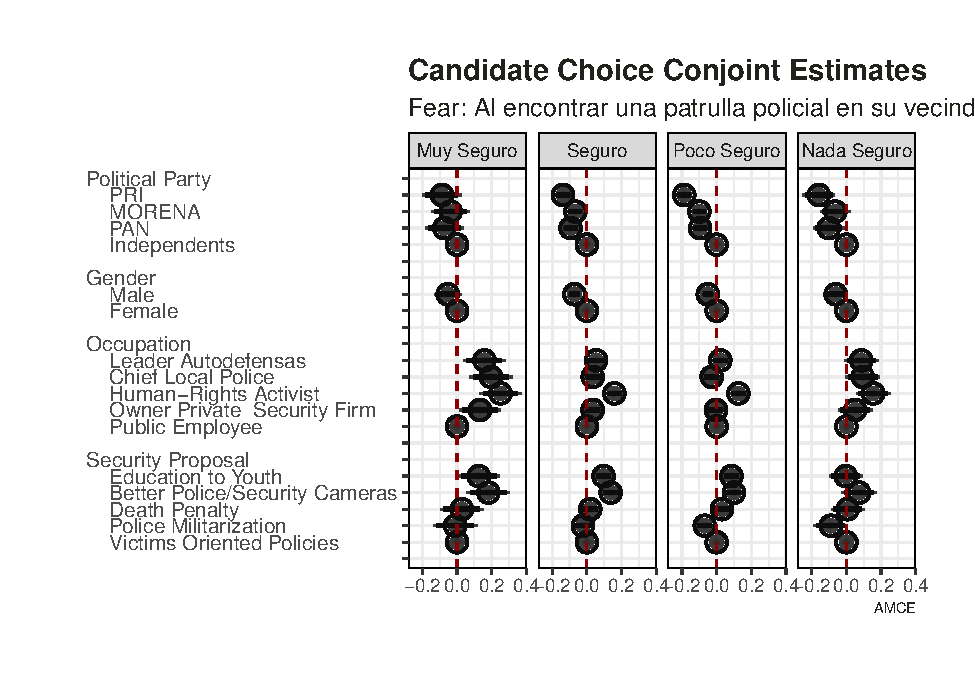
\includegraphics{report_conjoint_candidate_pdf_files/figure-latex/unnamed-chunk-7-4.pdf}

\hypertarget{mano-dura-preferences}{%
\subsection{Mano Dura Preferences}\label{mano-dura-preferences}}

\begin{Shaded}
\begin{Highlighting}[]
\CommentTok{# Law and Order -----------------------------------------------------------}
\KeywordTok{table}\NormalTok{(conjoint_data}\OperatorTok{$}\NormalTok{lo_}\DecValTok{1}\NormalTok{)}
\end{Highlighting}
\end{Shaded}

\begin{verbatim}

-999    0    1    3    4    5 
 859  916 1423 1548 2136 2321 
\end{verbatim}

\begin{Shaded}
\begin{Highlighting}[]
\CommentTok{# Recode}
\NormalTok{d_lo <-}\StringTok{ }\NormalTok{conjoint_data }\OperatorTok\StringTok{ }
\StringTok{  }\KeywordTok{mutate_at}\NormalTok{(}\KeywordTok{vars}\NormalTok{(lo_}\DecValTok{1}\NormalTok{, lo_}\DecValTok{2}\NormalTok{, lo_}\DecValTok{3}\NormalTok{, lo_}\DecValTok{4}\NormalTok{, lo_}\DecValTok{5}\NormalTok{), }\OperatorTok{~}\StringTok{ }
\StringTok{              }\KeywordTok{ifelse}\NormalTok{(.x }\OperatorTok\StringTok{ }\KeywordTok{c}\NormalTok{(}\StringTok{"-999"}\NormalTok{, }\StringTok{"No lo se"}\NormalTok{), }
                     \OtherTok{NA}\NormalTok{, .x)) }

\CommentTok{# Model}
\NormalTok{res_lo <-}\StringTok{ }\NormalTok{d_lo }\OperatorTok\StringTok{ }
\StringTok{  }\KeywordTok{group_by}\NormalTok{(lo_}\DecValTok{2}\NormalTok{) }\OperatorTok\StringTok{ }
\StringTok{  }\KeywordTok{nest}\NormalTok{() }\OperatorTok\StringTok{ }
\StringTok{  }\KeywordTok{drop_na}\NormalTok{() }\OperatorTok
\StringTok{  }\KeywordTok{mutate}\NormalTok{(}\DataTypeTok{model=}\KeywordTok{map2}\NormalTok{(data, lo_}\DecValTok{2}\NormalTok{, }
                    \OperatorTok{~}\StringTok{ }\KeywordTok{lm}\NormalTok{(outcome_num}\OperatorTok{~}\StringTok{ }\NormalTok{feat_political_party }\OperatorTok{+}\StringTok{ }\NormalTok{feat_gender }\OperatorTok{+}\StringTok{ }
\StringTok{                           }\NormalTok{feat_security_proposal }\OperatorTok{+}\StringTok{ }\NormalTok{feat_occupation, }
                         \DataTypeTok{data=}\NormalTok{.x) }\OperatorTok
\StringTok{                      }\KeywordTok{tidy_conjoint_model}\NormalTok{(}\DataTypeTok{model=}\NormalTok{., }\DataTypeTok{subsample=}\NormalTok{.y, }
                                          \DataTypeTok{features =}\NormalTok{ features,}
                                          \DataTypeTok{references=}\NormalTok{references, }\DataTypeTok{list_terms =}\NormalTok{ list_terms))) }\OperatorTok\StringTok{ }
\StringTok{  }\KeywordTok{unnest}\NormalTok{(model) }\OperatorTok\StringTok{ }\KeywordTok{select}\NormalTok{(}\OperatorTok{-}\NormalTok{data)}



\CommentTok{# # Remove repeated}
\CommentTok{# }
\CommentTok{# res_vict_color <- res_vict %>% ungroup() %>% }
\CommentTok{#   mutate(id_remove=ifelse(crime_victimization=="Victim"& (is.na(estimate) | estimate==0.0000), 1, 0),}
\CommentTok{#          crime_victimization=fct_rev(crime_victimization)) %>%}
\CommentTok{#   filter(id_remove==0) }


\KeywordTok{ggplot}\NormalTok{(res_lo, }\KeywordTok{aes}\NormalTok{(}\DataTypeTok{y=}\NormalTok{estimate, }\DataTypeTok{x=}\NormalTok{term, }
                     \DataTypeTok{ymin=}\NormalTok{up, }\DataTypeTok{ymax=}\NormalTok{lb)) }\OperatorTok{+}
\StringTok{  }\KeywordTok{geom_pointrange}\NormalTok{(}\DataTypeTok{size=}\NormalTok{.}\DecValTok{5}\NormalTok{, }\DataTypeTok{fill=}\StringTok{"black"}\NormalTok{, }\DataTypeTok{shape=}\DecValTok{21}\NormalTok{, }\DataTypeTok{color=}\StringTok{"grey5"}\NormalTok{,}
                  \DataTypeTok{position=}\KeywordTok{position_dodge}\NormalTok{(}\DataTypeTok{width =} \FloatTok{.6}\NormalTok{), }\DataTypeTok{alpha=}\NormalTok{.}\DecValTok{8}\NormalTok{) }\OperatorTok{+}
\StringTok{  }\KeywordTok{geom_pointrange}\NormalTok{(}\KeywordTok{aes}\NormalTok{(}\DataTypeTok{ymin=}\NormalTok{lb90, }\DataTypeTok{y=}\NormalTok{estimate, }\DataTypeTok{ymax=}\NormalTok{up90), }\DataTypeTok{shape=}\DecValTok{21}\NormalTok{, }
                  \DataTypeTok{size=}\DecValTok{1}\NormalTok{, }\DataTypeTok{color=}\StringTok{"grey5"}\NormalTok{) }\OperatorTok{+}
\StringTok{  }\KeywordTok{labs}\NormalTok{(}\DataTypeTok{x=}\StringTok{""}\NormalTok{, }\DataTypeTok{y=}\StringTok{"AMCE"}\NormalTok{, }
       \DataTypeTok{title =} \StringTok{"Candidate Choice Conjoint Estimates"}\NormalTok{, }
       \DataTypeTok{subtitle=}\StringTok{"Question: No Hay Mejor Ladron que el Ladron Muerto"}\NormalTok{) }\OperatorTok{+}
\StringTok{  }\KeywordTok{geom_hline}\NormalTok{(}\DataTypeTok{yintercept =} \DecValTok{0}\NormalTok{, }\DataTypeTok{linetype=}\StringTok{"dashed"}\NormalTok{, }\DataTypeTok{color=}\StringTok{"darkred"}\NormalTok{) }\OperatorTok{+}\StringTok{ }
\StringTok{  }\KeywordTok{scale_color_brewer}\NormalTok{(}\DataTypeTok{palette=}\StringTok{"Set1"}\NormalTok{) }\OperatorTok{+}
\StringTok{  }\KeywordTok{coord_flip}\NormalTok{() }\OperatorTok{+}\StringTok{ }
\StringTok{  }\KeywordTok{facet_grid}\NormalTok{(}\OperatorTok{~}\NormalTok{subsample)}\OperatorTok{+}\StringTok{ }
\StringTok{  }\KeywordTok{theme_bw}\NormalTok{()}\OperatorTok{+}\StringTok{ }\NormalTok{my_theme}
\end{Highlighting}
\end{Shaded}

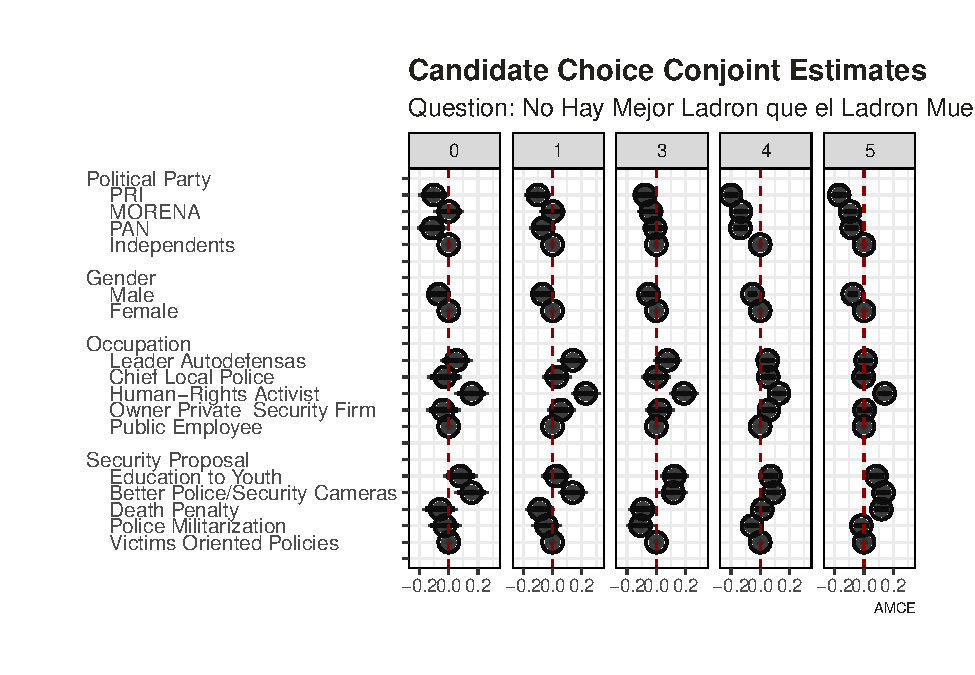
\includegraphics{report_conjoint_candidate_pdf_files/figure-latex/unnamed-chunk-8-1.pdf}

\end{document}
